% Options for packages loaded elsewhere
\PassOptionsToPackage{unicode}{hyperref}
\PassOptionsToPackage{hyphens}{url}
\PassOptionsToPackage{dvipsnames,svgnames,x11names}{xcolor}
%
\documentclass[
  letterpaper,
  DIV=11,
  numbers=noendperiod]{scrartcl}

\usepackage{amsmath,amssymb}
\usepackage{iftex}
\ifPDFTeX
  \usepackage[T1]{fontenc}
  \usepackage[utf8]{inputenc}
  \usepackage{textcomp} % provide euro and other symbols
\else % if luatex or xetex
  \usepackage{unicode-math}
  \defaultfontfeatures{Scale=MatchLowercase}
  \defaultfontfeatures[\rmfamily]{Ligatures=TeX,Scale=1}
\fi
\usepackage{lmodern}
\ifPDFTeX\else  
    % xetex/luatex font selection
\fi
% Use upquote if available, for straight quotes in verbatim environments
\IfFileExists{upquote.sty}{\usepackage{upquote}}{}
\IfFileExists{microtype.sty}{% use microtype if available
  \usepackage[]{microtype}
  \UseMicrotypeSet[protrusion]{basicmath} % disable protrusion for tt fonts
}{}
\makeatletter
\@ifundefined{KOMAClassName}{% if non-KOMA class
  \IfFileExists{parskip.sty}{%
    \usepackage{parskip}
  }{% else
    \setlength{\parindent}{0pt}
    \setlength{\parskip}{6pt plus 2pt minus 1pt}}
}{% if KOMA class
  \KOMAoptions{parskip=half}}
\makeatother
\usepackage{xcolor}
\setlength{\emergencystretch}{3em} % prevent overfull lines
\setcounter{secnumdepth}{5}
% Make \paragraph and \subparagraph free-standing
\makeatletter
\ifx\paragraph\undefined\else
  \let\oldparagraph\paragraph
  \renewcommand{\paragraph}{
    \@ifstar
      \xxxParagraphStar
      \xxxParagraphNoStar
  }
  \newcommand{\xxxParagraphStar}[1]{\oldparagraph*{#1}\mbox{}}
  \newcommand{\xxxParagraphNoStar}[1]{\oldparagraph{#1}\mbox{}}
\fi
\ifx\subparagraph\undefined\else
  \let\oldsubparagraph\subparagraph
  \renewcommand{\subparagraph}{
    \@ifstar
      \xxxSubParagraphStar
      \xxxSubParagraphNoStar
  }
  \newcommand{\xxxSubParagraphStar}[1]{\oldsubparagraph*{#1}\mbox{}}
  \newcommand{\xxxSubParagraphNoStar}[1]{\oldsubparagraph{#1}\mbox{}}
\fi
\makeatother

\usepackage{color}
\usepackage{fancyvrb}
\newcommand{\VerbBar}{|}
\newcommand{\VERB}{\Verb[commandchars=\\\{\}]}
\DefineVerbatimEnvironment{Highlighting}{Verbatim}{commandchars=\\\{\}}
% Add ',fontsize=\small' for more characters per line
\usepackage{framed}
\definecolor{shadecolor}{RGB}{241,243,245}
\newenvironment{Shaded}{\begin{snugshade}}{\end{snugshade}}
\newcommand{\AlertTok}[1]{\textcolor[rgb]{0.68,0.00,0.00}{#1}}
\newcommand{\AnnotationTok}[1]{\textcolor[rgb]{0.37,0.37,0.37}{#1}}
\newcommand{\AttributeTok}[1]{\textcolor[rgb]{0.40,0.45,0.13}{#1}}
\newcommand{\BaseNTok}[1]{\textcolor[rgb]{0.68,0.00,0.00}{#1}}
\newcommand{\BuiltInTok}[1]{\textcolor[rgb]{0.00,0.23,0.31}{#1}}
\newcommand{\CharTok}[1]{\textcolor[rgb]{0.13,0.47,0.30}{#1}}
\newcommand{\CommentTok}[1]{\textcolor[rgb]{0.37,0.37,0.37}{#1}}
\newcommand{\CommentVarTok}[1]{\textcolor[rgb]{0.37,0.37,0.37}{\textit{#1}}}
\newcommand{\ConstantTok}[1]{\textcolor[rgb]{0.56,0.35,0.01}{#1}}
\newcommand{\ControlFlowTok}[1]{\textcolor[rgb]{0.00,0.23,0.31}{\textbf{#1}}}
\newcommand{\DataTypeTok}[1]{\textcolor[rgb]{0.68,0.00,0.00}{#1}}
\newcommand{\DecValTok}[1]{\textcolor[rgb]{0.68,0.00,0.00}{#1}}
\newcommand{\DocumentationTok}[1]{\textcolor[rgb]{0.37,0.37,0.37}{\textit{#1}}}
\newcommand{\ErrorTok}[1]{\textcolor[rgb]{0.68,0.00,0.00}{#1}}
\newcommand{\ExtensionTok}[1]{\textcolor[rgb]{0.00,0.23,0.31}{#1}}
\newcommand{\FloatTok}[1]{\textcolor[rgb]{0.68,0.00,0.00}{#1}}
\newcommand{\FunctionTok}[1]{\textcolor[rgb]{0.28,0.35,0.67}{#1}}
\newcommand{\ImportTok}[1]{\textcolor[rgb]{0.00,0.46,0.62}{#1}}
\newcommand{\InformationTok}[1]{\textcolor[rgb]{0.37,0.37,0.37}{#1}}
\newcommand{\KeywordTok}[1]{\textcolor[rgb]{0.00,0.23,0.31}{\textbf{#1}}}
\newcommand{\NormalTok}[1]{\textcolor[rgb]{0.00,0.23,0.31}{#1}}
\newcommand{\OperatorTok}[1]{\textcolor[rgb]{0.37,0.37,0.37}{#1}}
\newcommand{\OtherTok}[1]{\textcolor[rgb]{0.00,0.23,0.31}{#1}}
\newcommand{\PreprocessorTok}[1]{\textcolor[rgb]{0.68,0.00,0.00}{#1}}
\newcommand{\RegionMarkerTok}[1]{\textcolor[rgb]{0.00,0.23,0.31}{#1}}
\newcommand{\SpecialCharTok}[1]{\textcolor[rgb]{0.37,0.37,0.37}{#1}}
\newcommand{\SpecialStringTok}[1]{\textcolor[rgb]{0.13,0.47,0.30}{#1}}
\newcommand{\StringTok}[1]{\textcolor[rgb]{0.13,0.47,0.30}{#1}}
\newcommand{\VariableTok}[1]{\textcolor[rgb]{0.07,0.07,0.07}{#1}}
\newcommand{\VerbatimStringTok}[1]{\textcolor[rgb]{0.13,0.47,0.30}{#1}}
\newcommand{\WarningTok}[1]{\textcolor[rgb]{0.37,0.37,0.37}{\textit{#1}}}

\providecommand{\tightlist}{%
  \setlength{\itemsep}{0pt}\setlength{\parskip}{0pt}}\usepackage{longtable,booktabs,array}
\usepackage{calc} % for calculating minipage widths
% Correct order of tables after \paragraph or \subparagraph
\usepackage{etoolbox}
\makeatletter
\patchcmd\longtable{\par}{\if@noskipsec\mbox{}\fi\par}{}{}
\makeatother
% Allow footnotes in longtable head/foot
\IfFileExists{footnotehyper.sty}{\usepackage{footnotehyper}}{\usepackage{footnote}}
\makesavenoteenv{longtable}
\usepackage{graphicx}
\makeatletter
\def\maxwidth{\ifdim\Gin@nat@width>\linewidth\linewidth\else\Gin@nat@width\fi}
\def\maxheight{\ifdim\Gin@nat@height>\textheight\textheight\else\Gin@nat@height\fi}
\makeatother
% Scale images if necessary, so that they will not overflow the page
% margins by default, and it is still possible to overwrite the defaults
% using explicit options in \includegraphics[width, height, ...]{}
\setkeys{Gin}{width=\maxwidth,height=\maxheight,keepaspectratio}
% Set default figure placement to htbp
\makeatletter
\def\fps@figure{htbp}
\makeatother

\KOMAoption{captions}{tableheading}
\makeatletter
\@ifpackageloaded{tcolorbox}{}{\usepackage[skins,breakable]{tcolorbox}}
\@ifpackageloaded{fontawesome5}{}{\usepackage{fontawesome5}}
\definecolor{quarto-callout-color}{HTML}{909090}
\definecolor{quarto-callout-note-color}{HTML}{0758E5}
\definecolor{quarto-callout-important-color}{HTML}{CC1914}
\definecolor{quarto-callout-warning-color}{HTML}{EB9113}
\definecolor{quarto-callout-tip-color}{HTML}{00A047}
\definecolor{quarto-callout-caution-color}{HTML}{FC5300}
\definecolor{quarto-callout-color-frame}{HTML}{acacac}
\definecolor{quarto-callout-note-color-frame}{HTML}{4582ec}
\definecolor{quarto-callout-important-color-frame}{HTML}{d9534f}
\definecolor{quarto-callout-warning-color-frame}{HTML}{f0ad4e}
\definecolor{quarto-callout-tip-color-frame}{HTML}{02b875}
\definecolor{quarto-callout-caution-color-frame}{HTML}{fd7e14}
\makeatother
\makeatletter
\@ifpackageloaded{caption}{}{\usepackage{caption}}
\AtBeginDocument{%
\ifdefined\contentsname
  \renewcommand*\contentsname{Table of contents}
\else
  \newcommand\contentsname{Table of contents}
\fi
\ifdefined\listfigurename
  \renewcommand*\listfigurename{List of Figures}
\else
  \newcommand\listfigurename{List of Figures}
\fi
\ifdefined\listtablename
  \renewcommand*\listtablename{List of Tables}
\else
  \newcommand\listtablename{List of Tables}
\fi
\ifdefined\figurename
  \renewcommand*\figurename{Figure}
\else
  \newcommand\figurename{Figure}
\fi
\ifdefined\tablename
  \renewcommand*\tablename{Table}
\else
  \newcommand\tablename{Table}
\fi
}
\@ifpackageloaded{float}{}{\usepackage{float}}
\floatstyle{ruled}
\@ifundefined{c@chapter}{\newfloat{codelisting}{h}{lop}}{\newfloat{codelisting}{h}{lop}[chapter]}
\floatname{codelisting}{Listing}
\newcommand*\listoflistings{\listof{codelisting}{List of Listings}}
\makeatother
\makeatletter
\makeatother
\makeatletter
\@ifpackageloaded{caption}{}{\usepackage{caption}}
\@ifpackageloaded{subcaption}{}{\usepackage{subcaption}}
\makeatother

\ifLuaTeX
  \usepackage{selnolig}  % disable illegal ligatures
\fi
\usepackage{bookmark}

\IfFileExists{xurl.sty}{\usepackage{xurl}}{} % add URL line breaks if available
\urlstyle{same} % disable monospaced font for URLs
\hypersetup{
  pdftitle={Palmer Penguins Data Analysis Series (Part 3): Advanced Models and Cross-Validation},
  pdfauthor={Your Name},
  colorlinks=true,
  linkcolor={blue},
  filecolor={Maroon},
  citecolor={Blue},
  urlcolor={Blue},
  pdfcreator={LaTeX via pandoc}}


\title{Palmer Penguins Data Analysis Series (Part 3): Advanced Models
and Cross-Validation}
\usepackage{etoolbox}
\makeatletter
\providecommand{\subtitle}[1]{% add subtitle to \maketitle
  \apptocmd{\@title}{\par {\large #1 \par}}{}{}
}
\makeatother
\subtitle{Testing model robustness and exploring the machine learning
frontier}
\author{Your Name}
\date{2025-01-03}

\begin{document}
\maketitle

\renewcommand*\contentsname{Table of contents}
{
\hypersetup{linkcolor=}
\setcounter{tocdepth}{3}
\tableofcontents
}

\begin{figure}[H]

{\centering 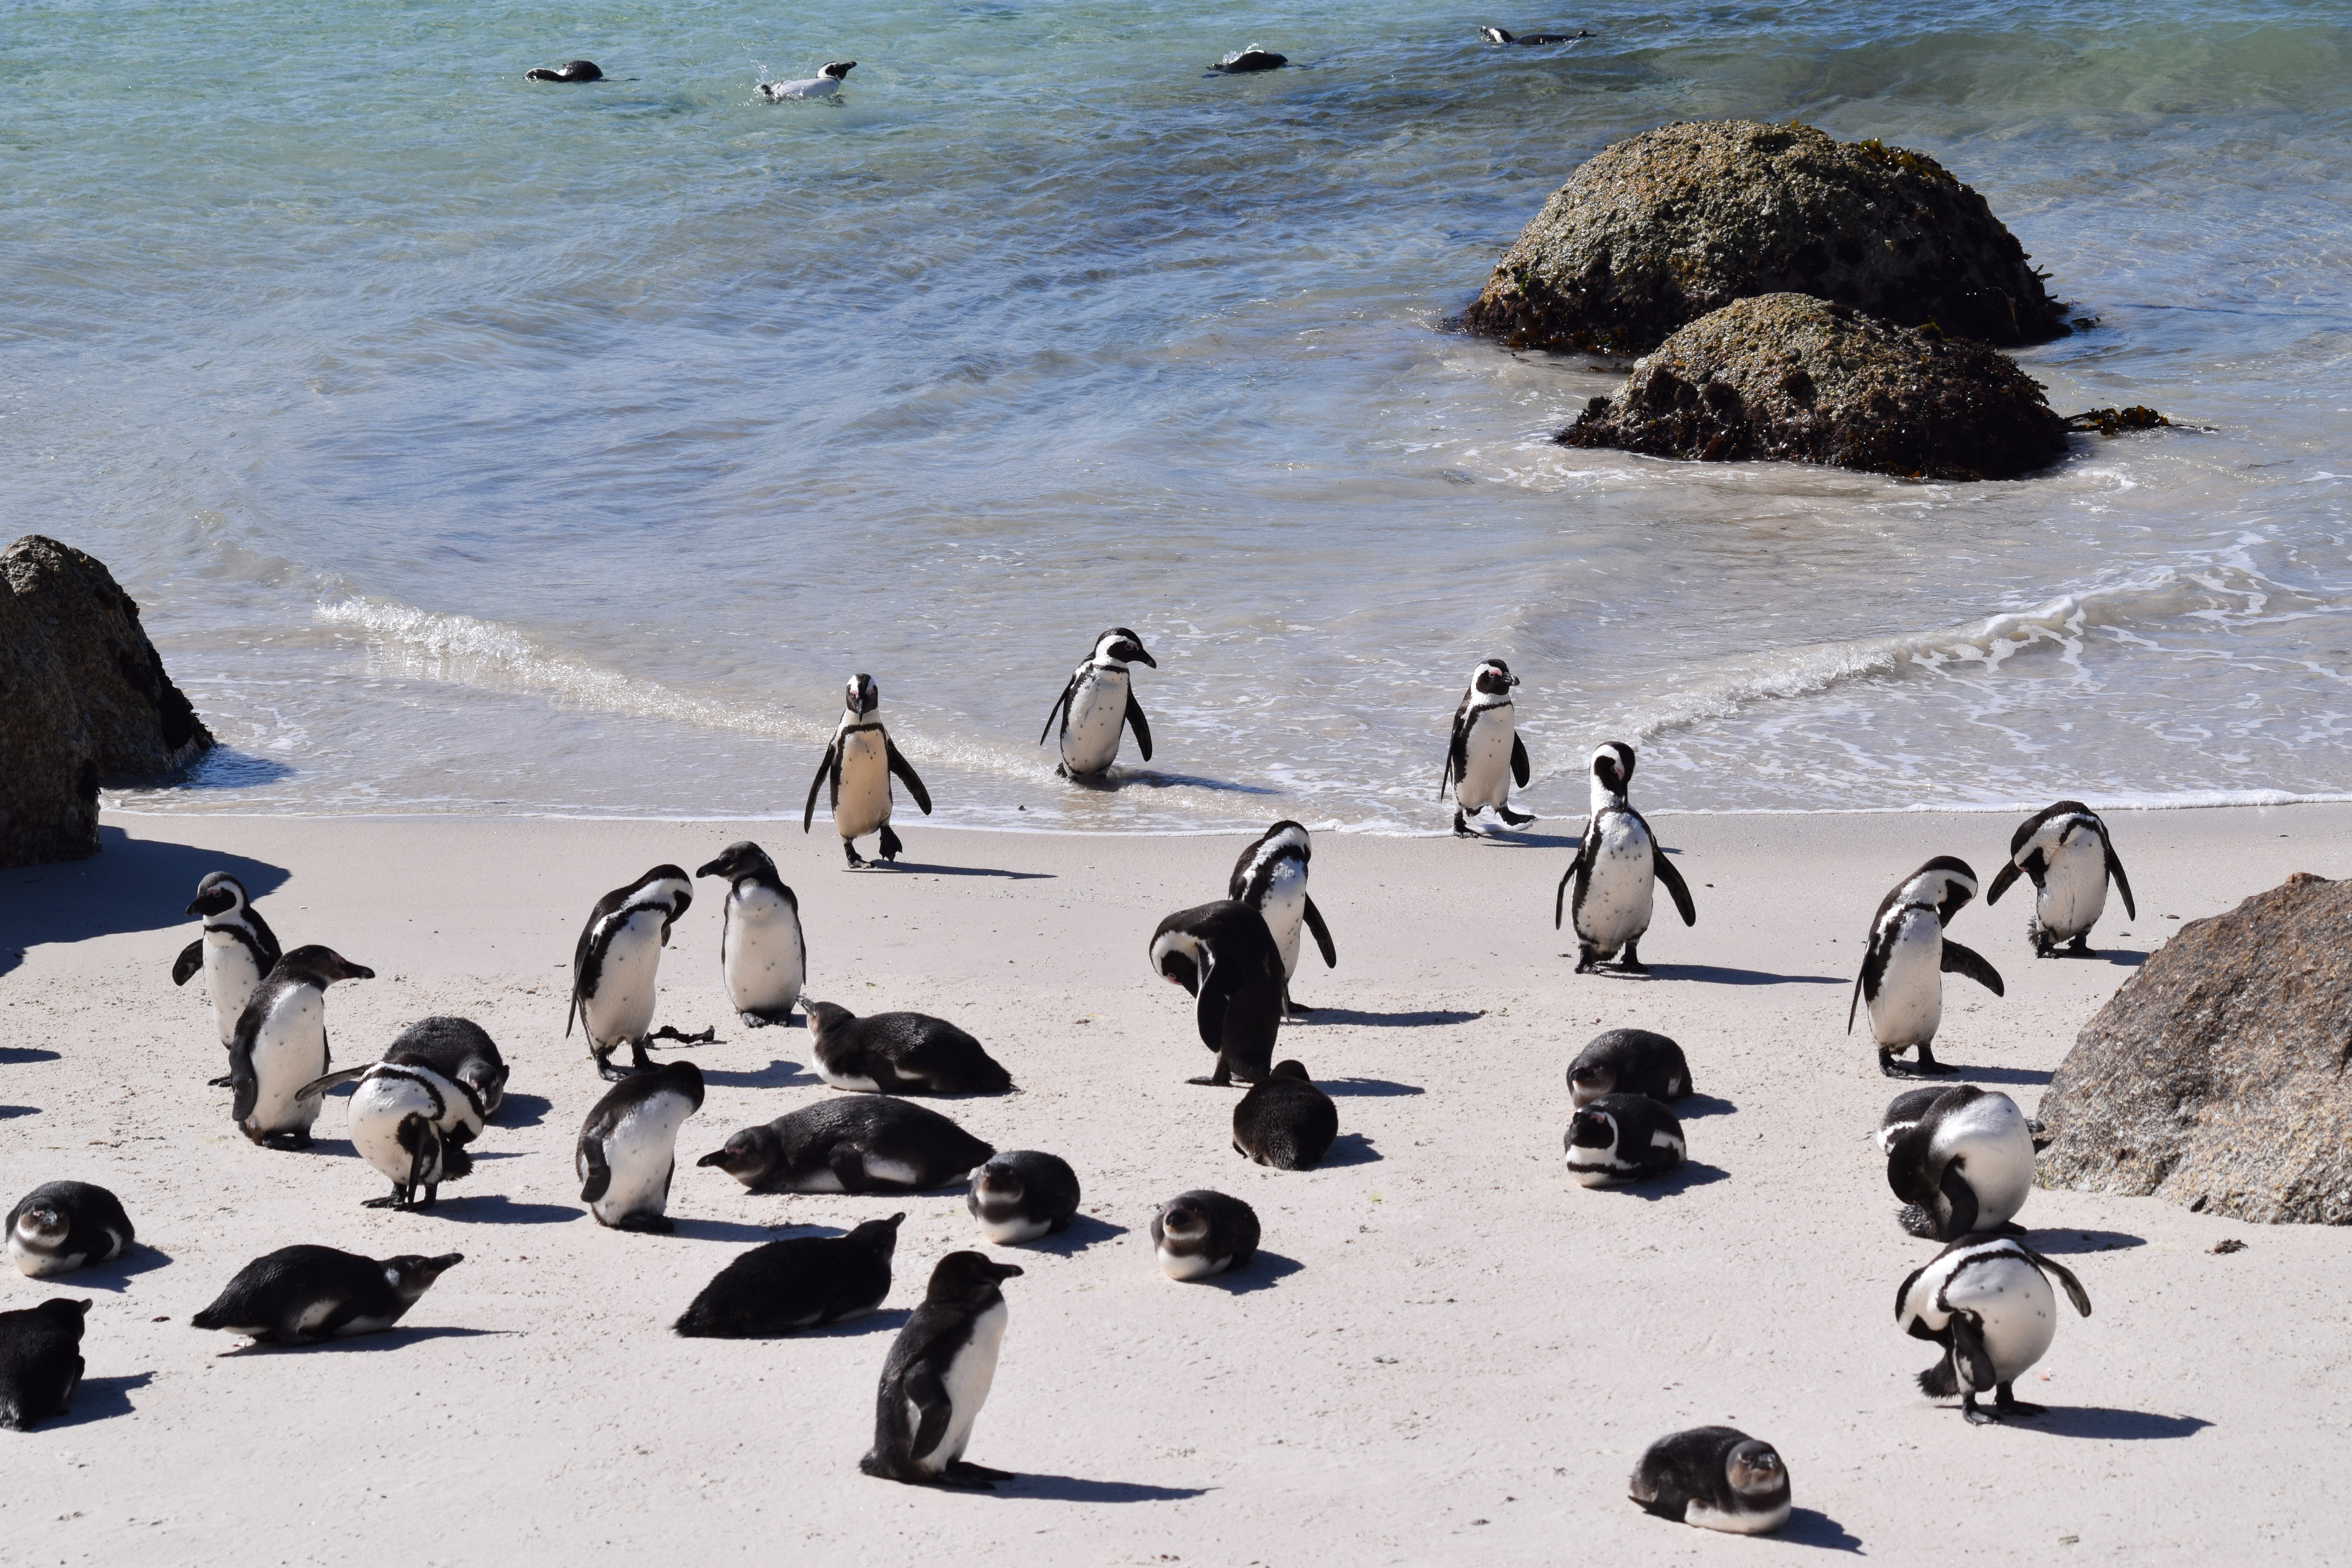
\includegraphics{../../images/posts/penguin-hero.jpg}

}

\caption{A tech-savvy penguin with a laptop, diving deep into advanced
modeling techniques and cross-validation!}

\end{figure}%

\emph{Photo: African penguins at Boulders Beach, South Africa. Licensed
under \href{https://creativecommons.org/licenses/by/2.0/}{CC BY 2.0} via
\href{https://commons.wikimedia.org/wiki/File:Boulders_Beach_penguins_(46475505885).jpg}{Wikimedia
Commons}}

\begin{tcolorbox}[enhanced jigsaw, opacityback=0, colframe=quarto-callout-note-color-frame, leftrule=.75mm, bottomrule=.15mm, left=2mm, toprule=.15mm, colback=white, breakable, rightrule=.15mm, arc=.35mm]
\begin{minipage}[t]{5.5mm}
\textcolor{quarto-callout-note-color}{\faInfo}
\end{minipage}%
\begin{minipage}[t]{\textwidth - 5.5mm}

\vspace{-3mm}\textbf{🐧 Palmer Penguins Data Analysis Series}\vspace{3mm}

This is \textbf{Part 3} of a 5-part series exploring penguin
morphometrics:

\begin{enumerate}
\def\labelenumi{\arabic{enumi}.}
\tightlist
\item
  \href{../palmer_penguins_part1/}{Part 1: EDA and Simple Regression}
\item
  \href{../palmer_penguins_part2/}{Part 2: Multiple Regression and
  Species Effects}
\item
  \textbf{Part 3: Advanced Models and Cross-Validation} (This post)
\item
  \href{../palmer_penguins_part4/}{Part 4: Model Diagnostics and
  Interpretation}
\item
  \href{../palmer_penguins_part5/}{Part 5: Random Forest vs Linear
  Models}
\end{enumerate}

\end{minipage}%
\end{tcolorbox}

\section{Introduction}\label{introduction}

Welcome to the third installment of our Palmer penguins adventure! In
\href{../palmer_penguins_part2/}{Part 2}, we achieved remarkable
results, boosting our R² from 76\% to 86\% by incorporating species
information. But as any responsible data scientist knows, impressive
performance on training data is only the beginning of the story.

The critical question remains: \textbf{How well will our models perform
on new, unseen penguin data?} This is where rigorous validation
techniques become essential. Today, we'll put our models through their
paces using cross-validation, explore whether non-linear relationships
can improve our predictions, and introduce our first machine learning
competitor.

In this post, we'll explore:

\begin{itemize}
\tightlist
\item
  Cross-validation techniques for robust model evaluation
\item
  Polynomial features to capture non-linear relationships\\
\item
  Random forest models as a machine learning baseline
\item
  Systematic model comparison with proper uncertainty quantification
\item
  The bias-variance tradeoff in action
\end{itemize}

By the end of this post, you'll have confidence in your model's
generalizability and understand when additional complexity helps versus
hurts predictive performance.

\section{Setup and Model Recap}\label{setup-and-model-recap}

Let's reload our work and establish our baseline models:

\begin{Shaded}
\begin{Highlighting}[]
\FunctionTok{library}\NormalTok{(palmerpenguins)}
\FunctionTok{library}\NormalTok{(tidyverse)}
\FunctionTok{library}\NormalTok{(broom)}
\CommentTok{\# Conditional loading of car package}
\ControlFlowTok{if}\NormalTok{ (}\FunctionTok{requireNamespace}\NormalTok{(}\StringTok{"car"}\NormalTok{, }\AttributeTok{quietly =} \ConstantTok{TRUE}\NormalTok{)) \{}
  \FunctionTok{library}\NormalTok{(car)}
\NormalTok{\} }\ControlFlowTok{else}\NormalTok{ \{}
  \FunctionTok{cat}\NormalTok{(}\StringTok{"⚠️ Package \textquotesingle{}car\textquotesingle{} not available. Install with: install.packages(\textquotesingle{}car\textquotesingle{})}\SpecialCharTok{\textbackslash{}n}\StringTok{"}\NormalTok{)}
\NormalTok{\}}
\FunctionTok{library}\NormalTok{(randomForest)}
\FunctionTok{library}\NormalTok{(caret)}
\FunctionTok{library}\NormalTok{(knitr)}
\FunctionTok{library}\NormalTok{(patchwork)}

\CommentTok{\# Set theme and colors}
\FunctionTok{theme\_set}\NormalTok{(}\FunctionTok{theme\_minimal}\NormalTok{(}\AttributeTok{base\_size =} \DecValTok{12}\NormalTok{))}
\NormalTok{penguin\_colors }\OtherTok{\textless{}{-}} \FunctionTok{c}\NormalTok{(}\StringTok{"Adelie"} \OtherTok{=} \StringTok{"\#FF6B6B"}\NormalTok{, }\StringTok{"Chinstrap"} \OtherTok{=} \StringTok{"\#4ECDC4"}\NormalTok{, }\StringTok{"Gentoo"} \OtherTok{=} \StringTok{"\#45B7D1"}\NormalTok{)}

\CommentTok{\# Load clean data}
\FunctionTok{data}\NormalTok{(penguins)}
\NormalTok{penguins\_clean }\OtherTok{\textless{}{-}}\NormalTok{ penguins }\SpecialCharTok{\%\textgreater{}\%} \FunctionTok{drop\_na}\NormalTok{()}

\CommentTok{\# Recreate our key models from previous parts}
\NormalTok{simple\_model }\OtherTok{\textless{}{-}} \FunctionTok{lm}\NormalTok{(body\_mass\_g }\SpecialCharTok{\textasciitilde{}}\NormalTok{ flipper\_length\_mm, }\AttributeTok{data =}\NormalTok{ penguins\_clean)}
\NormalTok{multiple\_model }\OtherTok{\textless{}{-}} \FunctionTok{lm}\NormalTok{(body\_mass\_g }\SpecialCharTok{\textasciitilde{}}\NormalTok{ bill\_length\_mm }\SpecialCharTok{+}\NormalTok{ bill\_depth\_mm }\SpecialCharTok{+}\NormalTok{ flipper\_length\_mm, }
                     \AttributeTok{data =}\NormalTok{ penguins\_clean)}
\NormalTok{species\_model }\OtherTok{\textless{}{-}} \FunctionTok{lm}\NormalTok{(body\_mass\_g }\SpecialCharTok{\textasciitilde{}}\NormalTok{ bill\_length\_mm }\SpecialCharTok{+}\NormalTok{ bill\_depth\_mm }\SpecialCharTok{+} 
\NormalTok{                    flipper\_length\_mm }\SpecialCharTok{+}\NormalTok{ species, }\AttributeTok{data =}\NormalTok{ penguins\_clean)}

\FunctionTok{cat}\NormalTok{(}\StringTok{"📋 Baseline Model Performance (Training Data):}\SpecialCharTok{\textbackslash{}n}\StringTok{"}\NormalTok{)}
\end{Highlighting}
\end{Shaded}

\begin{verbatim}
📋 Baseline Model Performance (Training Data):
\end{verbatim}

\begin{Shaded}
\begin{Highlighting}[]
\FunctionTok{cat}\NormalTok{(}\StringTok{"===============================================}\SpecialCharTok{\textbackslash{}n}\StringTok{"}\NormalTok{)}
\end{Highlighting}
\end{Shaded}

\begin{verbatim}
===============================================
\end{verbatim}

\begin{Shaded}
\begin{Highlighting}[]
\FunctionTok{cat}\NormalTok{(}\FunctionTok{sprintf}\NormalTok{(}\StringTok{"Simple model R²: \%.3f}\SpecialCharTok{\textbackslash{}n}\StringTok{"}\NormalTok{, }\FunctionTok{glance}\NormalTok{(simple\_model)}\SpecialCharTok{$}\NormalTok{r.squared))}
\end{Highlighting}
\end{Shaded}

\begin{verbatim}
Simple model R²: 0.762
\end{verbatim}

\begin{Shaded}
\begin{Highlighting}[]
\FunctionTok{cat}\NormalTok{(}\FunctionTok{sprintf}\NormalTok{(}\StringTok{"Multiple model R²: \%.3f}\SpecialCharTok{\textbackslash{}n}\StringTok{"}\NormalTok{, }\FunctionTok{glance}\NormalTok{(multiple\_model)}\SpecialCharTok{$}\NormalTok{r.squared))}
\end{Highlighting}
\end{Shaded}

\begin{verbatim}
Multiple model R²: 0.764
\end{verbatim}

\begin{Shaded}
\begin{Highlighting}[]
\FunctionTok{cat}\NormalTok{(}\FunctionTok{sprintf}\NormalTok{(}\StringTok{"Species model R²: \%.3f}\SpecialCharTok{\textbackslash{}n}\StringTok{"}\NormalTok{, }\FunctionTok{glance}\NormalTok{(species\_model)}\SpecialCharTok{$}\NormalTok{r.squared))}
\end{Highlighting}
\end{Shaded}

\begin{verbatim}
Species model R²: 0.849
\end{verbatim}

\begin{Shaded}
\begin{Highlighting}[]
\FunctionTok{cat}\NormalTok{(}\FunctionTok{sprintf}\NormalTok{(}\StringTok{"Sample size: \%d penguins}\SpecialCharTok{\textbackslash{}n}\StringTok{"}\NormalTok{, }\FunctionTok{nrow}\NormalTok{(penguins\_clean)))}
\end{Highlighting}
\end{Shaded}

\begin{verbatim}
Sample size: 333 penguins
\end{verbatim}

\section{Cross-Validation Framework}\label{cross-validation-framework}

Training performance can be misleading due to overfitting. Let's
implement k-fold cross-validation to get robust performance estimates:

\subsection{Setting Up
Cross-Validation}\label{setting-up-cross-validation}

\begin{Shaded}
\begin{Highlighting}[]
\FunctionTok{set.seed}\NormalTok{(}\DecValTok{42}\NormalTok{)  }\CommentTok{\# For reproducible results}

\CommentTok{\# Set up 10{-}fold cross{-}validation}
\NormalTok{train\_control }\OtherTok{\textless{}{-}} \FunctionTok{trainControl}\NormalTok{(}
  \AttributeTok{method =} \StringTok{"cv"}\NormalTok{,}
  \AttributeTok{number =} \DecValTok{10}\NormalTok{,}
  \AttributeTok{savePredictions =} \StringTok{"final"}\NormalTok{,}
  \AttributeTok{verboseIter =} \ConstantTok{FALSE}
\NormalTok{)}

\FunctionTok{cat}\NormalTok{(}\StringTok{"🔄 Cross{-}Validation Setup:}\SpecialCharTok{\textbackslash{}n}\StringTok{"}\NormalTok{)}
\end{Highlighting}
\end{Shaded}

\begin{verbatim}
🔄 Cross-Validation Setup:
\end{verbatim}

\begin{Shaded}
\begin{Highlighting}[]
\FunctionTok{cat}\NormalTok{(}\StringTok{"==========================}\SpecialCharTok{\textbackslash{}n}\StringTok{"}\NormalTok{)}
\end{Highlighting}
\end{Shaded}

\begin{verbatim}
==========================
\end{verbatim}

\begin{Shaded}
\begin{Highlighting}[]
\FunctionTok{cat}\NormalTok{(}\StringTok{"Method: 10{-}fold cross{-}validation}\SpecialCharTok{\textbackslash{}n}\StringTok{"}\NormalTok{)}
\end{Highlighting}
\end{Shaded}

\begin{verbatim}
Method: 10-fold cross-validation
\end{verbatim}

\begin{Shaded}
\begin{Highlighting}[]
\FunctionTok{cat}\NormalTok{(}\StringTok{"Folds: 10}\SpecialCharTok{\textbackslash{}n}\StringTok{"}\NormalTok{)}
\end{Highlighting}
\end{Shaded}

\begin{verbatim}
Folds: 10
\end{verbatim}

\begin{Shaded}
\begin{Highlighting}[]
\FunctionTok{cat}\NormalTok{(}\StringTok{"Seed: 42 (for reproducibility)}\SpecialCharTok{\textbackslash{}n}\StringTok{"}\NormalTok{)}
\end{Highlighting}
\end{Shaded}

\begin{verbatim}
Seed: 42 (for reproducibility)
\end{verbatim}

\begin{Shaded}
\begin{Highlighting}[]
\FunctionTok{cat}\NormalTok{(}\StringTok{"Predictions saved: Yes}\SpecialCharTok{\textbackslash{}n}\StringTok{"}\NormalTok{)}
\end{Highlighting}
\end{Shaded}

\begin{verbatim}
Predictions saved: Yes
\end{verbatim}

\subsection{Cross-Validating Our Existing
Models}\label{cross-validating-our-existing-models}

\begin{Shaded}
\begin{Highlighting}[]
\CommentTok{\# Cross{-}validate simple model}
\NormalTok{cv\_simple }\OtherTok{\textless{}{-}} \FunctionTok{train}\NormalTok{(}
\NormalTok{  body\_mass\_g }\SpecialCharTok{\textasciitilde{}}\NormalTok{ flipper\_length\_mm,}
  \AttributeTok{data =}\NormalTok{ penguins\_clean,}
  \AttributeTok{method =} \StringTok{"lm"}\NormalTok{,}
  \AttributeTok{trControl =}\NormalTok{ train\_control}
\NormalTok{)}

\CommentTok{\# Cross{-}validate multiple regression model}
\NormalTok{cv\_multiple }\OtherTok{\textless{}{-}} \FunctionTok{train}\NormalTok{(}
\NormalTok{  body\_mass\_g }\SpecialCharTok{\textasciitilde{}}\NormalTok{ bill\_length\_mm }\SpecialCharTok{+}\NormalTok{ bill\_depth\_mm }\SpecialCharTok{+}\NormalTok{ flipper\_length\_mm,}
  \AttributeTok{data =}\NormalTok{ penguins\_clean,}
  \AttributeTok{method =} \StringTok{"lm"}\NormalTok{, }
  \AttributeTok{trControl =}\NormalTok{ train\_control}
\NormalTok{)}

\CommentTok{\# Cross{-}validate species model}
\NormalTok{cv\_species }\OtherTok{\textless{}{-}} \FunctionTok{train}\NormalTok{(}
\NormalTok{  body\_mass\_g }\SpecialCharTok{\textasciitilde{}}\NormalTok{ bill\_length\_mm }\SpecialCharTok{+}\NormalTok{ bill\_depth\_mm }\SpecialCharTok{+}\NormalTok{ flipper\_length\_mm }\SpecialCharTok{+}\NormalTok{ species,}
  \AttributeTok{data =}\NormalTok{ penguins\_clean,}
  \AttributeTok{method =} \StringTok{"lm"}\NormalTok{,}
  \AttributeTok{trControl =}\NormalTok{ train\_control}
\NormalTok{)}

\CommentTok{\# Display cross{-}validation results}
\FunctionTok{cat}\NormalTok{(}\StringTok{"}\SpecialCharTok{\textbackslash{}n}\StringTok{📊 Cross{-}Validation Results:}\SpecialCharTok{\textbackslash{}n}\StringTok{"}\NormalTok{)}
\end{Highlighting}
\end{Shaded}

\begin{verbatim}

📊 Cross-Validation Results:
\end{verbatim}

\begin{Shaded}
\begin{Highlighting}[]
\FunctionTok{cat}\NormalTok{(}\StringTok{"=============================}\SpecialCharTok{\textbackslash{}n}\StringTok{"}\NormalTok{)}
\end{Highlighting}
\end{Shaded}

\begin{verbatim}
=============================
\end{verbatim}

\begin{Shaded}
\begin{Highlighting}[]
\FunctionTok{cat}\NormalTok{(}\FunctionTok{sprintf}\NormalTok{(}\StringTok{"Simple model {-} RMSE: \%.1f (±\%.1f), R²: \%.3f (±\%.3f)}\SpecialCharTok{\textbackslash{}n}\StringTok{"}\NormalTok{,}
\NormalTok{            cv\_simple}\SpecialCharTok{$}\NormalTok{results}\SpecialCharTok{$}\NormalTok{RMSE, }\FunctionTok{sd}\NormalTok{(cv\_simple}\SpecialCharTok{$}\NormalTok{resample}\SpecialCharTok{$}\NormalTok{RMSE),}
\NormalTok{            cv\_simple}\SpecialCharTok{$}\NormalTok{results}\SpecialCharTok{$}\NormalTok{Rsquared, }\FunctionTok{sd}\NormalTok{(cv\_simple}\SpecialCharTok{$}\NormalTok{resample}\SpecialCharTok{$}\NormalTok{Rsquared)))}
\end{Highlighting}
\end{Shaded}

\begin{verbatim}
Simple model - RMSE: 390.9 (±54.0), R²: 0.775 (±0.038)
\end{verbatim}

\begin{Shaded}
\begin{Highlighting}[]
\FunctionTok{cat}\NormalTok{(}\FunctionTok{sprintf}\NormalTok{(}\StringTok{"Multiple model {-} RMSE: \%.1f (±\%.1f), R²: \%.3f (±\%.3f)}\SpecialCharTok{\textbackslash{}n}\StringTok{"}\NormalTok{,}
\NormalTok{            cv\_multiple}\SpecialCharTok{$}\NormalTok{results}\SpecialCharTok{$}\NormalTok{RMSE, }\FunctionTok{sd}\NormalTok{(cv\_multiple}\SpecialCharTok{$}\NormalTok{resample}\SpecialCharTok{$}\NormalTok{RMSE),}
\NormalTok{            cv\_multiple}\SpecialCharTok{$}\NormalTok{results}\SpecialCharTok{$}\NormalTok{Rsquared, }\FunctionTok{sd}\NormalTok{(cv\_multiple}\SpecialCharTok{$}\NormalTok{resample}\SpecialCharTok{$}\NormalTok{Rsquared)))}
\end{Highlighting}
\end{Shaded}

\begin{verbatim}
Multiple model - RMSE: 392.6 (±41.7), R²: 0.769 (±0.049)
\end{verbatim}

\begin{Shaded}
\begin{Highlighting}[]
\FunctionTok{cat}\NormalTok{(}\FunctionTok{sprintf}\NormalTok{(}\StringTok{"Species model {-} RMSE: \%.1f (±\%.1f), R²: \%.3f (±\%.3f)}\SpecialCharTok{\textbackslash{}n}\StringTok{"}\NormalTok{,}
\NormalTok{            cv\_species}\SpecialCharTok{$}\NormalTok{results}\SpecialCharTok{$}\NormalTok{RMSE, }\FunctionTok{sd}\NormalTok{(cv\_species}\SpecialCharTok{$}\NormalTok{resample}\SpecialCharTok{$}\NormalTok{RMSE),}
\NormalTok{            cv\_species}\SpecialCharTok{$}\NormalTok{results}\SpecialCharTok{$}\NormalTok{Rsquared, }\FunctionTok{sd}\NormalTok{(cv\_species}\SpecialCharTok{$}\NormalTok{resample}\SpecialCharTok{$}\NormalTok{Rsquared)))}
\end{Highlighting}
\end{Shaded}

\begin{verbatim}
Species model - RMSE: 315.7 (±32.2), R²: 0.856 (±0.022)
\end{verbatim}

\subsection{Visualizing Cross-Validation
Results}\label{visualizing-cross-validation-results}

\begin{Shaded}
\begin{Highlighting}[]
\CommentTok{\# Create comprehensive CV results dataframe}
\NormalTok{cv\_results }\OtherTok{\textless{}{-}} \FunctionTok{data.frame}\NormalTok{(}
  \AttributeTok{Model =} \FunctionTok{rep}\NormalTok{(}\FunctionTok{c}\NormalTok{(}\StringTok{"Simple"}\NormalTok{, }\StringTok{"Multiple"}\NormalTok{, }\StringTok{"Species"}\NormalTok{), }\AttributeTok{each =} \DecValTok{10}\NormalTok{),}
  \AttributeTok{RMSE =} \FunctionTok{c}\NormalTok{(cv\_simple}\SpecialCharTok{$}\NormalTok{resample}\SpecialCharTok{$}\NormalTok{RMSE, cv\_multiple}\SpecialCharTok{$}\NormalTok{resample}\SpecialCharTok{$}\NormalTok{RMSE, cv\_species}\SpecialCharTok{$}\NormalTok{resample}\SpecialCharTok{$}\NormalTok{RMSE),}
  \AttributeTok{Rsquared =} \FunctionTok{c}\NormalTok{(cv\_simple}\SpecialCharTok{$}\NormalTok{resample}\SpecialCharTok{$}\NormalTok{Rsquared, cv\_multiple}\SpecialCharTok{$}\NormalTok{resample}\SpecialCharTok{$}\NormalTok{Rsquared, cv\_species}\SpecialCharTok{$}\NormalTok{resample}\SpecialCharTok{$}\NormalTok{Rsquared)}
\NormalTok{)}

\CommentTok{\# Box plots of CV performance}
\NormalTok{p1 }\OtherTok{\textless{}{-}} \FunctionTok{ggplot}\NormalTok{(cv\_results, }\FunctionTok{aes}\NormalTok{(}\AttributeTok{x =}\NormalTok{ Model, }\AttributeTok{y =}\NormalTok{ RMSE, }\AttributeTok{fill =}\NormalTok{ Model)) }\SpecialCharTok{+}
  \FunctionTok{geom\_boxplot}\NormalTok{(}\AttributeTok{alpha =} \FloatTok{0.7}\NormalTok{) }\SpecialCharTok{+}
  \FunctionTok{geom\_jitter}\NormalTok{(}\AttributeTok{width =} \FloatTok{0.2}\NormalTok{, }\AttributeTok{alpha =} \FloatTok{0.5}\NormalTok{) }\SpecialCharTok{+}
  \FunctionTok{labs}\NormalTok{(}\AttributeTok{title =} \StringTok{"Cross{-}Validation RMSE Distribution"}\NormalTok{,}
       \AttributeTok{subtitle =} \StringTok{"Lower values indicate better performance"}\NormalTok{,}
       \AttributeTok{y =} \StringTok{"RMSE (grams)"}\NormalTok{) }\SpecialCharTok{+}
  \FunctionTok{theme}\NormalTok{(}\AttributeTok{legend.position =} \StringTok{"none"}\NormalTok{)}

\NormalTok{p2 }\OtherTok{\textless{}{-}} \FunctionTok{ggplot}\NormalTok{(cv\_results, }\FunctionTok{aes}\NormalTok{(}\AttributeTok{x =}\NormalTok{ Model, }\AttributeTok{y =}\NormalTok{ Rsquared, }\AttributeTok{fill =}\NormalTok{ Model)) }\SpecialCharTok{+}
  \FunctionTok{geom\_boxplot}\NormalTok{(}\AttributeTok{alpha =} \FloatTok{0.7}\NormalTok{) }\SpecialCharTok{+}
  \FunctionTok{geom\_jitter}\NormalTok{(}\AttributeTok{width =} \FloatTok{0.2}\NormalTok{, }\AttributeTok{alpha =} \FloatTok{0.5}\NormalTok{) }\SpecialCharTok{+}
  \FunctionTok{labs}\NormalTok{(}\AttributeTok{title =} \StringTok{"Cross{-}Validation R² Distribution"}\NormalTok{, }
       \AttributeTok{subtitle =} \StringTok{"Higher values indicate better performance"}\NormalTok{,}
       \AttributeTok{y =} \StringTok{"R{-}squared"}\NormalTok{) }\SpecialCharTok{+}
  \FunctionTok{theme}\NormalTok{(}\AttributeTok{legend.position =} \StringTok{"none"}\NormalTok{)}

\NormalTok{cv\_performance\_plot }\OtherTok{\textless{}{-}}\NormalTok{ p1 }\SpecialCharTok{+}\NormalTok{ p2}
\FunctionTok{print}\NormalTok{(cv\_performance\_plot)}
\end{Highlighting}
\end{Shaded}

\includegraphics{index_files/figure-pdf/unnamed-chunk-4-1.pdf}

\begin{figure}[H]

{\centering \includegraphics{cv-performance-distribution.png}

}

\caption{Box plots showing the distribution of cross-validation
performance metrics across folds}

\end{figure}%

\section{Polynomial Features}\label{polynomial-features}

Linear relationships might not capture all the complexity in biological
data. Let's explore polynomial features:

\subsection{Adding Quadratic Terms}\label{adding-quadratic-terms}

\begin{Shaded}
\begin{Highlighting}[]
\CommentTok{\# Create polynomial model with quadratic terms}
\NormalTok{poly\_model }\OtherTok{\textless{}{-}} \FunctionTok{lm}\NormalTok{(body\_mass\_g }\SpecialCharTok{\textasciitilde{}} \FunctionTok{poly}\NormalTok{(flipper\_length\_mm, }\DecValTok{2}\NormalTok{) }\SpecialCharTok{+} \FunctionTok{poly}\NormalTok{(bill\_length\_mm, }\DecValTok{2}\NormalTok{) }\SpecialCharTok{+} 
                 \FunctionTok{poly}\NormalTok{(bill\_depth\_mm, }\DecValTok{2}\NormalTok{) }\SpecialCharTok{+}\NormalTok{ species, }\AttributeTok{data =}\NormalTok{ penguins\_clean)}

\FunctionTok{summary}\NormalTok{(poly\_model)}
\end{Highlighting}
\end{Shaded}

\begin{verbatim}

Call:
lm(formula = body_mass_g ~ poly(flipper_length_mm, 2) + poly(bill_length_mm, 
    2) + poly(bill_depth_mm, 2) + species, data = penguins_clean)

Residuals:
    Min      1Q  Median      3Q     Max 
-837.68 -209.78  -25.97  187.14 1012.84 

Coefficients:
                            Estimate Std. Error t value Pr(>|t|)    
(Intercept)                  3935.52      69.77  56.404  < 2e-16 ***
poly(flipper_length_mm, 2)1  5321.73     859.97   6.188 1.84e-09 ***
poly(flipper_length_mm, 2)2   391.41     407.10   0.961   0.3370    
poly(bill_length_mm, 2)1     3753.51     726.72   5.165 4.21e-07 ***
poly(bill_length_mm, 2)2     -856.40     345.09  -2.482   0.0136 *  
poly(bill_depth_mm, 2)1      5764.01     769.85   7.487 6.72e-13 ***
poly(bill_depth_mm, 2)2      -842.97     404.23  -2.085   0.0378 *  
speciesChinstrap             -470.97      84.01  -5.606 4.43e-08 ***
speciesGentoo                1028.96     161.74   6.362 6.79e-10 ***
---
Signif. codes:  0 '***' 0.001 '**' 0.01 '*' 0.05 '.' 0.1 ' ' 1

Residual standard error: 310.1 on 324 degrees of freedom
Multiple R-squared:  0.8552,    Adjusted R-squared:  0.8516 
F-statistic: 239.2 on 8 and 324 DF,  p-value: < 2.2e-16
\end{verbatim}

\begin{Shaded}
\begin{Highlighting}[]
\CommentTok{\# Cross{-}validate polynomial model}
\NormalTok{cv\_poly }\OtherTok{\textless{}{-}} \FunctionTok{train}\NormalTok{(}
\NormalTok{  body\_mass\_g }\SpecialCharTok{\textasciitilde{}} \FunctionTok{poly}\NormalTok{(flipper\_length\_mm, }\DecValTok{2}\NormalTok{) }\SpecialCharTok{+} \FunctionTok{poly}\NormalTok{(bill\_length\_mm, }\DecValTok{2}\NormalTok{) }\SpecialCharTok{+} 
                \FunctionTok{poly}\NormalTok{(bill\_depth\_mm, }\DecValTok{2}\NormalTok{) }\SpecialCharTok{+}\NormalTok{ species,}
  \AttributeTok{data =}\NormalTok{ penguins\_clean,}
  \AttributeTok{method =} \StringTok{"lm"}\NormalTok{,}
  \AttributeTok{trControl =}\NormalTok{ train\_control}
\NormalTok{)}

\FunctionTok{cat}\NormalTok{(}\StringTok{"🔄 Polynomial Model Cross{-}Validation:}\SpecialCharTok{\textbackslash{}n}\StringTok{"}\NormalTok{)}
\end{Highlighting}
\end{Shaded}

\begin{verbatim}
🔄 Polynomial Model Cross-Validation:
\end{verbatim}

\begin{Shaded}
\begin{Highlighting}[]
\FunctionTok{cat}\NormalTok{(}\StringTok{"=====================================}\SpecialCharTok{\textbackslash{}n}\StringTok{"}\NormalTok{)}
\end{Highlighting}
\end{Shaded}

\begin{verbatim}
=====================================
\end{verbatim}

\begin{Shaded}
\begin{Highlighting}[]
\FunctionTok{cat}\NormalTok{(}\FunctionTok{sprintf}\NormalTok{(}\StringTok{"Polynomial model {-} RMSE: \%.1f (±\%.1f), R²: \%.3f (±\%.3f)}\SpecialCharTok{\textbackslash{}n}\StringTok{"}\NormalTok{,}
\NormalTok{            cv\_poly}\SpecialCharTok{$}\NormalTok{results}\SpecialCharTok{$}\NormalTok{RMSE, }\FunctionTok{sd}\NormalTok{(cv\_poly}\SpecialCharTok{$}\NormalTok{resample}\SpecialCharTok{$}\NormalTok{RMSE),}
\NormalTok{            cv\_poly}\SpecialCharTok{$}\NormalTok{results}\SpecialCharTok{$}\NormalTok{Rsquared, }\FunctionTok{sd}\NormalTok{(cv\_poly}\SpecialCharTok{$}\NormalTok{resample}\SpecialCharTok{$}\NormalTok{Rsquared)))}
\end{Highlighting}
\end{Shaded}

\begin{verbatim}
Polynomial model - RMSE: 310.8 (±44.4), R²: 0.855 (±0.046)
\end{verbatim}

\subsection{Visualizing Non-linear
Relationships}\label{visualizing-non-linear-relationships}

\begin{Shaded}
\begin{Highlighting}[]
\CommentTok{\# Create predictions for visualization}
\NormalTok{flipper\_range }\OtherTok{\textless{}{-}} \FunctionTok{seq}\NormalTok{(}\FunctionTok{min}\NormalTok{(penguins\_clean}\SpecialCharTok{$}\NormalTok{flipper\_length\_mm), }
                     \FunctionTok{max}\NormalTok{(penguins\_clean}\SpecialCharTok{$}\NormalTok{flipper\_length\_mm), }\AttributeTok{length.out =} \DecValTok{100}\NormalTok{)}

\CommentTok{\# Compare linear vs polynomial relationships for each species}
\NormalTok{prediction\_data }\OtherTok{\textless{}{-}} \FunctionTok{expand\_grid}\NormalTok{(}
  \AttributeTok{flipper\_length\_mm =}\NormalTok{ flipper\_range,}
  \AttributeTok{species =} \FunctionTok{unique}\NormalTok{(penguins\_clean}\SpecialCharTok{$}\NormalTok{species)}
\NormalTok{) }\SpecialCharTok{\%\textgreater{}\%}
  \FunctionTok{mutate}\NormalTok{(}
    \AttributeTok{bill\_length\_mm =} \FunctionTok{mean}\NormalTok{(penguins\_clean}\SpecialCharTok{$}\NormalTok{bill\_length\_mm),}
    \AttributeTok{bill\_depth\_mm =} \FunctionTok{mean}\NormalTok{(penguins\_clean}\SpecialCharTok{$}\NormalTok{bill\_depth\_mm),}
    \AttributeTok{body\_mass\_g =} \DecValTok{0}  \CommentTok{\# placeholder}
\NormalTok{  )}

\CommentTok{\# Get predictions from both models}
\NormalTok{prediction\_data}\SpecialCharTok{$}\NormalTok{linear\_pred }\OtherTok{\textless{}{-}} \FunctionTok{predict}\NormalTok{(species\_model, }\AttributeTok{newdata =}\NormalTok{ prediction\_data)}
\NormalTok{prediction\_data}\SpecialCharTok{$}\NormalTok{poly\_pred }\OtherTok{\textless{}{-}} \FunctionTok{predict}\NormalTok{(poly\_model, }\AttributeTok{newdata =}\NormalTok{ prediction\_data)}

\CommentTok{\# Visualization}
\FunctionTok{ggplot}\NormalTok{(penguins\_clean, }\FunctionTok{aes}\NormalTok{(}\AttributeTok{x =}\NormalTok{ flipper\_length\_mm, }\AttributeTok{y =}\NormalTok{ body\_mass\_g, }\AttributeTok{color =}\NormalTok{ species)) }\SpecialCharTok{+}
  \FunctionTok{geom\_point}\NormalTok{(}\AttributeTok{alpha =} \FloatTok{0.6}\NormalTok{, }\AttributeTok{size =} \DecValTok{2}\NormalTok{) }\SpecialCharTok{+}
  \FunctionTok{geom\_line}\NormalTok{(}\AttributeTok{data =}\NormalTok{ prediction\_data, }\FunctionTok{aes}\NormalTok{(}\AttributeTok{y =}\NormalTok{ linear\_pred, }\AttributeTok{linetype =} \StringTok{"Linear"}\NormalTok{), }
            \AttributeTok{size =} \DecValTok{1}\NormalTok{, }\AttributeTok{alpha =} \FloatTok{0.8}\NormalTok{) }\SpecialCharTok{+}
  \FunctionTok{geom\_line}\NormalTok{(}\AttributeTok{data =}\NormalTok{ prediction\_data, }\FunctionTok{aes}\NormalTok{(}\AttributeTok{y =}\NormalTok{ poly\_pred, }\AttributeTok{linetype =} \StringTok{"Polynomial"}\NormalTok{), }
            \AttributeTok{size =} \DecValTok{1}\NormalTok{, }\AttributeTok{alpha =} \FloatTok{0.8}\NormalTok{) }\SpecialCharTok{+}
  \FunctionTok{scale\_color\_manual}\NormalTok{(}\AttributeTok{values =}\NormalTok{ penguin\_colors) }\SpecialCharTok{+}
  \FunctionTok{scale\_linetype\_manual}\NormalTok{(}\AttributeTok{values =} \FunctionTok{c}\NormalTok{(}\StringTok{"Linear"} \OtherTok{=} \StringTok{"dashed"}\NormalTok{, }\StringTok{"Polynomial"} \OtherTok{=} \StringTok{"solid"}\NormalTok{)) }\SpecialCharTok{+}
  \FunctionTok{labs}\NormalTok{(}\AttributeTok{title =} \StringTok{"Linear vs Polynomial Relationships"}\NormalTok{,}
       \AttributeTok{subtitle =} \StringTok{"Comparing model fits for flipper length (other variables held at mean)"}\NormalTok{,}
       \AttributeTok{x =} \StringTok{"Flipper Length (mm)"}\NormalTok{, }\AttributeTok{y =} \StringTok{"Body Mass (g)"}\NormalTok{,}
       \AttributeTok{color =} \StringTok{"Species"}\NormalTok{, }\AttributeTok{linetype =} \StringTok{"Model"}\NormalTok{) }\SpecialCharTok{+}
  \FunctionTok{facet\_wrap}\NormalTok{(}\SpecialCharTok{\textasciitilde{}}\NormalTok{species) }\SpecialCharTok{+}
  \FunctionTok{theme\_minimal}\NormalTok{()}
\end{Highlighting}
\end{Shaded}

\includegraphics{index_files/figure-pdf/unnamed-chunk-6-1.pdf}

\begin{figure}[H]

{\centering \includegraphics{linear-vs-polynomial.png}

}

\caption{Comparison of linear versus polynomial model fits across
species}

\end{figure}%

\section{Random Forest Models}\label{random-forest-models}

Now let's introduce our first machine learning approach - random
forests:

\subsection{Basic Random Forest}\label{basic-random-forest}

\begin{Shaded}
\begin{Highlighting}[]
\FunctionTok{set.seed}\NormalTok{(}\DecValTok{123}\NormalTok{)}

\CommentTok{\# Train random forest using caret for consistency}
\NormalTok{cv\_rf }\OtherTok{\textless{}{-}} \FunctionTok{train}\NormalTok{(}
\NormalTok{  body\_mass\_g }\SpecialCharTok{\textasciitilde{}}\NormalTok{ bill\_length\_mm }\SpecialCharTok{+}\NormalTok{ bill\_depth\_mm }\SpecialCharTok{+}\NormalTok{ flipper\_length\_mm }\SpecialCharTok{+}\NormalTok{ species }\SpecialCharTok{+}\NormalTok{ sex }\SpecialCharTok{+}\NormalTok{ island,}
  \AttributeTok{data =}\NormalTok{ penguins\_clean,}
  \AttributeTok{method =} \StringTok{"rf"}\NormalTok{,}
  \AttributeTok{trControl =}\NormalTok{ train\_control,}
  \AttributeTok{ntree =} \DecValTok{500}\NormalTok{,}
  \AttributeTok{importance =} \ConstantTok{TRUE}
\NormalTok{)}

\FunctionTok{print}\NormalTok{(cv\_rf)}
\end{Highlighting}
\end{Shaded}

\begin{verbatim}
Random Forest 

333 samples
  6 predictor

No pre-processing
Resampling: Cross-Validated (10 fold) 
Summary of sample sizes: 299, 300, 300, 300, 299, 300, ... 
Resampling results across tuning parameters:

  mtry  RMSE      Rsquared   MAE     
  2     296.1693  0.8709290  235.7196
  5     300.8044  0.8666035  239.2056
  8     304.0154  0.8638966  242.7076

RMSE was used to select the optimal model using the smallest value.
The final value used for the model was mtry = 2.
\end{verbatim}

\begin{Shaded}
\begin{Highlighting}[]
\FunctionTok{cat}\NormalTok{(}\StringTok{"}\SpecialCharTok{\textbackslash{}n}\StringTok{🌲 Random Forest Cross{-}Validation:}\SpecialCharTok{\textbackslash{}n}\StringTok{"}\NormalTok{)}
\end{Highlighting}
\end{Shaded}

\begin{verbatim}

🌲 Random Forest Cross-Validation:
\end{verbatim}

\begin{Shaded}
\begin{Highlighting}[]
\FunctionTok{cat}\NormalTok{(}\StringTok{"===================================}\SpecialCharTok{\textbackslash{}n}\StringTok{"}\NormalTok{)}
\end{Highlighting}
\end{Shaded}

\begin{verbatim}
===================================
\end{verbatim}

\begin{Shaded}
\begin{Highlighting}[]
\FunctionTok{cat}\NormalTok{(}\FunctionTok{sprintf}\NormalTok{(}\StringTok{"Random Forest {-} RMSE: \%.1f (±\%.1f), R²: \%.3f (±\%.3f)}\SpecialCharTok{\textbackslash{}n}\StringTok{"}\NormalTok{,}
            \FunctionTok{min}\NormalTok{(cv\_rf}\SpecialCharTok{$}\NormalTok{results}\SpecialCharTok{$}\NormalTok{RMSE), }\FunctionTok{sd}\NormalTok{(cv\_rf}\SpecialCharTok{$}\NormalTok{resample}\SpecialCharTok{$}\NormalTok{RMSE),}
            \FunctionTok{max}\NormalTok{(cv\_rf}\SpecialCharTok{$}\NormalTok{results}\SpecialCharTok{$}\NormalTok{Rsquared), }\FunctionTok{sd}\NormalTok{(cv\_rf}\SpecialCharTok{$}\NormalTok{resample}\SpecialCharTok{$}\NormalTok{Rsquared)))}
\end{Highlighting}
\end{Shaded}

\begin{verbatim}
Random Forest - RMSE: 296.2 (±40.5), R²: 0.871 (±0.032)
\end{verbatim}

\subsection{Variable Importance}\label{variable-importance}

\begin{Shaded}
\begin{Highlighting}[]
\CommentTok{\# Extract variable importance}
\NormalTok{rf\_importance }\OtherTok{\textless{}{-}} \FunctionTok{varImp}\NormalTok{(cv\_rf)}
\FunctionTok{print}\NormalTok{(rf\_importance)}
\end{Highlighting}
\end{Shaded}

\begin{verbatim}
rf variable importance

                  Overall
sexmale            100.00
speciesGentoo       68.83
bill_depth_mm       68.63
flipper_length_mm   61.96
bill_length_mm      45.02
islandDream         27.56
speciesChinstrap    17.01
islandTorgersen      0.00
\end{verbatim}

\begin{Shaded}
\begin{Highlighting}[]
\CommentTok{\# Visualize importance}
\NormalTok{importance\_plot }\OtherTok{\textless{}{-}} \FunctionTok{ggplot}\NormalTok{(rf\_importance) }\SpecialCharTok{+}
  \FunctionTok{labs}\NormalTok{(}\AttributeTok{title =} \StringTok{"Random Forest Variable Importance"}\NormalTok{,}
       \AttributeTok{subtitle =} \StringTok{"Relative contribution to prediction accuracy"}\NormalTok{) }\SpecialCharTok{+}
  \FunctionTok{theme\_minimal}\NormalTok{()}

\FunctionTok{print}\NormalTok{(importance\_plot)}
\end{Highlighting}
\end{Shaded}

\includegraphics{index_files/figure-pdf/unnamed-chunk-8-1.pdf}

\begin{figure}[H]

{\centering \includegraphics{rf-variable-importance.png}

}

\caption{Variable importance plot showing which features contribute most
to random forest predictions}

\end{figure}%

\section{Comprehensive Model
Comparison}\label{comprehensive-model-comparison}

Let's create a complete comparison of all our models:

\subsection{Performance Summary Table}\label{performance-summary-table}

\begin{Shaded}
\begin{Highlighting}[]
\CommentTok{\# Compile all cross{-}validation results}
\NormalTok{all\_models }\OtherTok{\textless{}{-}} \FunctionTok{list}\NormalTok{(}
  \StringTok{"Simple"} \OtherTok{=}\NormalTok{ cv\_simple,}
  \StringTok{"Multiple"} \OtherTok{=}\NormalTok{ cv\_multiple, }
  \StringTok{"Species"} \OtherTok{=}\NormalTok{ cv\_species,}
  \StringTok{"Polynomial"} \OtherTok{=}\NormalTok{ cv\_poly,}
  \StringTok{"Random Forest"} \OtherTok{=}\NormalTok{ cv\_rf}
\NormalTok{)}

\CommentTok{\# Extract performance metrics}
\NormalTok{model\_performance }\OtherTok{\textless{}{-}} \FunctionTok{map\_dfr}\NormalTok{(all\_models, }\ControlFlowTok{function}\NormalTok{(model) \{}
  \FunctionTok{data.frame}\NormalTok{(}
    \AttributeTok{RMSE\_mean =} \FunctionTok{min}\NormalTok{(model}\SpecialCharTok{$}\NormalTok{results}\SpecialCharTok{$}\NormalTok{RMSE),}
    \AttributeTok{RMSE\_sd =} \FunctionTok{sd}\NormalTok{(model}\SpecialCharTok{$}\NormalTok{resample}\SpecialCharTok{$}\NormalTok{RMSE),}
    \AttributeTok{Rsquared\_mean =} \FunctionTok{max}\NormalTok{(model}\SpecialCharTok{$}\NormalTok{results}\SpecialCharTok{$}\NormalTok{Rsquared),}
    \AttributeTok{Rsquared\_sd =} \FunctionTok{sd}\NormalTok{(model}\SpecialCharTok{$}\NormalTok{resample}\SpecialCharTok{$}\NormalTok{Rsquared),}
    \AttributeTok{MAE\_mean =} \FunctionTok{min}\NormalTok{(model}\SpecialCharTok{$}\NormalTok{results}\SpecialCharTok{$}\NormalTok{MAE)}
\NormalTok{  )}
\NormalTok{\}, }\AttributeTok{.id =} \StringTok{"Model"}\NormalTok{) }\SpecialCharTok{\%\textgreater{}\%}
  \FunctionTok{arrange}\NormalTok{(RMSE\_mean)}

\CommentTok{\# Format for display}
\NormalTok{model\_performance\_display }\OtherTok{\textless{}{-}}\NormalTok{ model\_performance }\SpecialCharTok{\%\textgreater{}\%}
  \FunctionTok{mutate}\NormalTok{(}
    \AttributeTok{RMSE =} \FunctionTok{sprintf}\NormalTok{(}\StringTok{"\%.1f ± \%.1f"}\NormalTok{, RMSE\_mean, RMSE\_sd),}
    \AttributeTok{R\_squared =} \FunctionTok{sprintf}\NormalTok{(}\StringTok{"\%.3f ± \%.3f"}\NormalTok{, Rsquared\_mean, Rsquared\_sd),}
    \AttributeTok{MAE =} \FunctionTok{sprintf}\NormalTok{(}\StringTok{"\%.1f"}\NormalTok{, MAE\_mean)}
\NormalTok{  ) }\SpecialCharTok{\%\textgreater{}\%}
  \FunctionTok{select}\NormalTok{(Model, RMSE, R\_squared, MAE)}

\FunctionTok{kable}\NormalTok{(model\_performance\_display,}
      \AttributeTok{caption =} \StringTok{"Cross{-}Validation Performance Comparison (Mean ± Standard Deviation)"}\NormalTok{,}
      \AttributeTok{col.names =} \FunctionTok{c}\NormalTok{(}\StringTok{"Model"}\NormalTok{, }\StringTok{"RMSE (g)"}\NormalTok{, }\StringTok{"R²"}\NormalTok{, }\StringTok{"MAE (g)"}\NormalTok{))}
\end{Highlighting}
\end{Shaded}

\begin{longtable}[]{@{}llll@{}}
\caption{Cross-Validation Performance Comparison (Mean ± Standard
Deviation)}\tabularnewline
\toprule\noalign{}
Model & RMSE (g) & R² & MAE (g) \\
\midrule\noalign{}
\endfirsthead
\toprule\noalign{}
Model & RMSE (g) & R² & MAE (g) \\
\midrule\noalign{}
\endhead
\bottomrule\noalign{}
\endlastfoot
Random Forest & 296.2 ± 40.5 & 0.871 ± 0.032 & 235.7 \\
Polynomial & 310.8 ± 44.4 & 0.855 ± 0.046 & 249.8 \\
Species & 315.7 ± 32.2 & 0.856 ± 0.022 & 251.6 \\
Simple & 390.9 ± 54.0 & 0.775 ± 0.038 & 314.1 \\
Multiple & 392.6 ± 41.7 & 0.769 ± 0.049 & 312.9 \\
\end{longtable}

\subsection{Statistical Significance
Testing}\label{statistical-significance-testing}

\begin{Shaded}
\begin{Highlighting}[]
\CommentTok{\# Perform pairwise comparisons using resamples}
\NormalTok{model\_resamples }\OtherTok{\textless{}{-}} \FunctionTok{resamples}\NormalTok{(all\_models)}
\FunctionTok{summary}\NormalTok{(model\_resamples)}
\end{Highlighting}
\end{Shaded}

\begin{verbatim}

Call:
summary.resamples(object = model_resamples)

Models: Simple, Multiple, Species, Polynomial, Random Forest 
Number of resamples: 10 

MAE 
                  Min.  1st Qu.   Median     Mean  3rd Qu.     Max. NA's
Simple        241.3554 284.0399 320.8430 314.0739 338.4259 371.1883    0
Multiple      260.4224 299.3261 312.0693 312.9230 324.2053 361.2878    0
Species       221.3089 229.2132 249.0898 251.5796 266.4538 291.5125    0
Polynomial    202.4456 230.6144 239.4014 249.8384 260.2454 339.3528    0
Random Forest 160.8733 216.7519 228.7049 235.7196 262.9530 294.3425    0

RMSE 
                  Min.  1st Qu.   Median     Mean  3rd Qu.     Max. NA's
Simple        308.6200 349.3536 401.5457 390.8672 426.1235 458.9253    0
Multiple      313.5602 370.9372 386.3221 392.6475 414.3106 459.0243    0
Species       272.3076 291.1982 314.1444 315.7035 345.0607 357.2340    0
Polynomial    240.1316 291.2401 311.3770 310.8124 332.1709 397.4275    0
Random Forest 219.6603 272.3759 290.9904 296.1693 332.7067 345.1353    0

Rsquared 
                   Min.   1st Qu.    Median      Mean   3rd Qu.      Max. NA's
Simple        0.7338776 0.7504191 0.7629768 0.7753345 0.7986835 0.8402682    0
Multiple      0.6868671 0.7275708 0.7928215 0.7690730 0.7998317 0.8242159    0
Species       0.8296272 0.8381939 0.8522291 0.8558827 0.8744437 0.8906614    0
Polynomial    0.7579544 0.8363657 0.8517021 0.8548061 0.8848488 0.9257512    0
Random Forest 0.8231393 0.8479029 0.8780378 0.8709290 0.8823033 0.9407561    0
\end{verbatim}

\begin{Shaded}
\begin{Highlighting}[]
\CommentTok{\# Statistical comparison}
\NormalTok{model\_differences }\OtherTok{\textless{}{-}} \FunctionTok{diff}\NormalTok{(model\_resamples)}
\FunctionTok{summary}\NormalTok{(model\_differences)}
\end{Highlighting}
\end{Shaded}

\begin{verbatim}

Call:
summary.diff.resamples(object = model_differences)

p-value adjustment: bonferroni 
Upper diagonal: estimates of the difference
Lower diagonal: p-value for H0: difference = 0

MAE 
              Simple   Multiple Species  Polynomial Random Forest
Simple                  1.151   62.494   64.235     78.354       
Multiple      1.000000          61.343   63.085     77.203       
Species       0.073024 0.002911           1.741     15.860       
Polynomial    0.052589 0.003403 1.000000            14.119       
Random Forest 0.031252 0.002025 1.000000 1.000000                

RMSE 
              Simple   Multiple Species  Polynomial Random Forest
Simple                 -1.780   75.164   80.055     94.698       
Multiple      1.000000          76.944   81.835     96.478       
Species       0.089778 0.013250           4.891     19.534       
Polynomial    0.050086 0.001917 1.000000            14.643       
Random Forest 0.013082 0.000986 1.000000 1.000000                

Rsquared 
              Simple   Multiple  Species   Polynomial Random Forest
Simple                  0.006262 -0.080548 -0.079472  -0.095594    
Multiple      1.000000           -0.086810 -0.085733  -0.101856    
Species       0.008511 0.006787             0.001077  -0.015046    
Polynomial    0.061015 0.004296  1.000000             -0.016123    
Random Forest 0.001177 0.002549  1.000000  1.000000                
\end{verbatim}

\subsection{Performance Visualization}\label{performance-visualization}

\begin{Shaded}
\begin{Highlighting}[]
\CommentTok{\# Create comprehensive comparison plot}
\NormalTok{all\_cv\_results }\OtherTok{\textless{}{-}} \FunctionTok{data.frame}\NormalTok{(}
  \AttributeTok{Model =} \FunctionTok{factor}\NormalTok{(}\FunctionTok{rep}\NormalTok{(}\FunctionTok{names}\NormalTok{(all\_models), }\AttributeTok{each =} \DecValTok{10}\NormalTok{), }\AttributeTok{levels =} \FunctionTok{names}\NormalTok{(all\_models)),}
  \AttributeTok{RMSE =} \FunctionTok{c}\NormalTok{(cv\_simple}\SpecialCharTok{$}\NormalTok{resample}\SpecialCharTok{$}\NormalTok{RMSE, cv\_multiple}\SpecialCharTok{$}\NormalTok{resample}\SpecialCharTok{$}\NormalTok{RMSE, }
\NormalTok{           cv\_species}\SpecialCharTok{$}\NormalTok{resample}\SpecialCharTok{$}\NormalTok{RMSE, cv\_poly}\SpecialCharTok{$}\NormalTok{resample}\SpecialCharTok{$}\NormalTok{RMSE, cv\_rf}\SpecialCharTok{$}\NormalTok{resample}\SpecialCharTok{$}\NormalTok{RMSE),}
  \AttributeTok{Rsquared =} \FunctionTok{c}\NormalTok{(cv\_simple}\SpecialCharTok{$}\NormalTok{resample}\SpecialCharTok{$}\NormalTok{Rsquared, cv\_multiple}\SpecialCharTok{$}\NormalTok{resample}\SpecialCharTok{$}\NormalTok{Rsquared,}
\NormalTok{               cv\_species}\SpecialCharTok{$}\NormalTok{resample}\SpecialCharTok{$}\NormalTok{Rsquared, cv\_poly}\SpecialCharTok{$}\NormalTok{resample}\SpecialCharTok{$}\NormalTok{Rsquared, cv\_rf}\SpecialCharTok{$}\NormalTok{resample}\SpecialCharTok{$}\NormalTok{Rsquared)}
\NormalTok{)}

\CommentTok{\# RMSE comparison}
\NormalTok{p3 }\OtherTok{\textless{}{-}} \FunctionTok{ggplot}\NormalTok{(all\_cv\_results, }\FunctionTok{aes}\NormalTok{(}\AttributeTok{x =}\NormalTok{ Model, }\AttributeTok{y =}\NormalTok{ RMSE, }\AttributeTok{fill =}\NormalTok{ Model)) }\SpecialCharTok{+}
  \FunctionTok{geom\_boxplot}\NormalTok{(}\AttributeTok{alpha =} \FloatTok{0.7}\NormalTok{) }\SpecialCharTok{+}
  \FunctionTok{stat\_summary}\NormalTok{(}\AttributeTok{fun =}\NormalTok{ mean, }\AttributeTok{geom =} \StringTok{"point"}\NormalTok{, }\AttributeTok{shape =} \DecValTok{23}\NormalTok{, }\AttributeTok{size =} \DecValTok{3}\NormalTok{, }\AttributeTok{fill =} \StringTok{"white"}\NormalTok{) }\SpecialCharTok{+}
  \FunctionTok{labs}\NormalTok{(}\AttributeTok{title =} \StringTok{"Cross{-}Validation RMSE Comparison"}\NormalTok{,}
       \AttributeTok{subtitle =} \StringTok{"Lower is better; white diamonds show means"}\NormalTok{,}
       \AttributeTok{y =} \StringTok{"RMSE (grams)"}\NormalTok{) }\SpecialCharTok{+}
  \FunctionTok{theme}\NormalTok{(}\AttributeTok{axis.text.x =} \FunctionTok{element\_text}\NormalTok{(}\AttributeTok{angle =} \DecValTok{45}\NormalTok{, }\AttributeTok{hjust =} \DecValTok{1}\NormalTok{), }\AttributeTok{legend.position =} \StringTok{"none"}\NormalTok{)}

\CommentTok{\# R² comparison  }
\NormalTok{p4 }\OtherTok{\textless{}{-}} \FunctionTok{ggplot}\NormalTok{(all\_cv\_results, }\FunctionTok{aes}\NormalTok{(}\AttributeTok{x =}\NormalTok{ Model, }\AttributeTok{y =}\NormalTok{ Rsquared, }\AttributeTok{fill =}\NormalTok{ Model)) }\SpecialCharTok{+}
  \FunctionTok{geom\_boxplot}\NormalTok{(}\AttributeTok{alpha =} \FloatTok{0.7}\NormalTok{) }\SpecialCharTok{+}
  \FunctionTok{stat\_summary}\NormalTok{(}\AttributeTok{fun =}\NormalTok{ mean, }\AttributeTok{geom =} \StringTok{"point"}\NormalTok{, }\AttributeTok{shape =} \DecValTok{23}\NormalTok{, }\AttributeTok{size =} \DecValTok{3}\NormalTok{, }\AttributeTok{fill =} \StringTok{"white"}\NormalTok{) }\SpecialCharTok{+}
  \FunctionTok{labs}\NormalTok{(}\AttributeTok{title =} \StringTok{"Cross{-}Validation R² Comparison"}\NormalTok{,}
       \AttributeTok{subtitle =} \StringTok{"Higher is better; white diamonds show means"}\NormalTok{, }
       \AttributeTok{y =} \StringTok{"R{-}squared"}\NormalTok{) }\SpecialCharTok{+}
  \FunctionTok{theme}\NormalTok{(}\AttributeTok{axis.text.x =} \FunctionTok{element\_text}\NormalTok{(}\AttributeTok{angle =} \DecValTok{45}\NormalTok{, }\AttributeTok{hjust =} \DecValTok{1}\NormalTok{), }\AttributeTok{legend.position =} \StringTok{"none"}\NormalTok{)}

\NormalTok{comprehensive\_comparison }\OtherTok{\textless{}{-}}\NormalTok{ p3 }\SpecialCharTok{+}\NormalTok{ p4}
\FunctionTok{print}\NormalTok{(comprehensive\_comparison)}
\end{Highlighting}
\end{Shaded}

\includegraphics{index_files/figure-pdf/unnamed-chunk-11-1.pdf}

\begin{figure}[H]

{\centering \includegraphics{comprehensive-model-comparison.png}

}

\caption{Comprehensive comparison of all models showing both RMSE and R²
distributions from cross-validation}

\end{figure}%

\section{The Bias-Variance Tradeoff}\label{the-bias-variance-tradeoff}

Let's examine how model complexity affects the bias-variance tradeoff:

\subsection{Learning Curves}\label{learning-curves}

\begin{Shaded}
\begin{Highlighting}[]
\CommentTok{\# Function to calculate learning curves}
\NormalTok{calculate\_learning\_curve }\OtherTok{\textless{}{-}} \ControlFlowTok{function}\NormalTok{(model\_formula, data, }\AttributeTok{train\_sizes =} \FunctionTok{seq}\NormalTok{(}\FloatTok{0.1}\NormalTok{, }\DecValTok{1}\NormalTok{, }\FloatTok{0.1}\NormalTok{)) \{}
\NormalTok{  results }\OtherTok{\textless{}{-}} \FunctionTok{map\_dfr}\NormalTok{(train\_sizes, }\ControlFlowTok{function}\NormalTok{(size) \{}
\NormalTok{    n\_train }\OtherTok{\textless{}{-}} \FunctionTok{round}\NormalTok{(}\FunctionTok{nrow}\NormalTok{(data) }\SpecialCharTok{*}\NormalTok{ size)}
    
    \CommentTok{\# Perform multiple bootstrap samples}
\NormalTok{    bootstrap\_results }\OtherTok{\textless{}{-}} \FunctionTok{map\_dfr}\NormalTok{(}\DecValTok{1}\SpecialCharTok{:}\DecValTok{20}\NormalTok{, }\ControlFlowTok{function}\NormalTok{(i) \{}
      \FunctionTok{set.seed}\NormalTok{(i)}
\NormalTok{      train\_idx }\OtherTok{\textless{}{-}} \FunctionTok{sample}\NormalTok{(}\FunctionTok{nrow}\NormalTok{(data), n\_train)}
\NormalTok{      train\_data }\OtherTok{\textless{}{-}}\NormalTok{ data[train\_idx, ]}
\NormalTok{      test\_data }\OtherTok{\textless{}{-}}\NormalTok{ data[}\SpecialCharTok{{-}}\NormalTok{train\_idx, ]}
      
      \CommentTok{\# Fit model}
\NormalTok{      model }\OtherTok{\textless{}{-}} \FunctionTok{lm}\NormalTok{(model\_formula, }\AttributeTok{data =}\NormalTok{ train\_data)}
      
      \CommentTok{\# Calculate errors}
\NormalTok{      train\_pred }\OtherTok{\textless{}{-}} \FunctionTok{predict}\NormalTok{(model, train\_data)}
\NormalTok{      test\_pred }\OtherTok{\textless{}{-}} \FunctionTok{predict}\NormalTok{(model, test\_data)}
      
      \FunctionTok{data.frame}\NormalTok{(}
        \AttributeTok{train\_size =}\NormalTok{ size,}
        \AttributeTok{train\_rmse =} \FunctionTok{sqrt}\NormalTok{(}\FunctionTok{mean}\NormalTok{((train\_data}\SpecialCharTok{$}\NormalTok{body\_mass\_g }\SpecialCharTok{{-}}\NormalTok{ train\_pred)}\SpecialCharTok{\^{}}\DecValTok{2}\NormalTok{)),}
        \AttributeTok{test\_rmse =} \ControlFlowTok{if}\NormalTok{(}\FunctionTok{nrow}\NormalTok{(test\_data) }\SpecialCharTok{\textgreater{}} \DecValTok{0}\NormalTok{) }\FunctionTok{sqrt}\NormalTok{(}\FunctionTok{mean}\NormalTok{((test\_data}\SpecialCharTok{$}\NormalTok{body\_mass\_g }\SpecialCharTok{{-}}\NormalTok{ test\_pred)}\SpecialCharTok{\^{}}\DecValTok{2}\NormalTok{)) }\ControlFlowTok{else} \ConstantTok{NA}\NormalTok{,}
        \AttributeTok{bootstrap =}\NormalTok{ i}
\NormalTok{      )}
\NormalTok{    \})}
    
\NormalTok{    bootstrap\_results}
\NormalTok{  \})}
  
\NormalTok{  results}
\NormalTok{\}}

\CommentTok{\# Calculate learning curves for key models}
\NormalTok{learning\_simple }\OtherTok{\textless{}{-}} \FunctionTok{calculate\_learning\_curve}\NormalTok{(}
\NormalTok{  body\_mass\_g }\SpecialCharTok{\textasciitilde{}}\NormalTok{ flipper\_length\_mm, penguins\_clean)}
\NormalTok{learning\_species }\OtherTok{\textless{}{-}} \FunctionTok{calculate\_learning\_curve}\NormalTok{(}
\NormalTok{  body\_mass\_g }\SpecialCharTok{\textasciitilde{}}\NormalTok{ bill\_length\_mm }\SpecialCharTok{+}\NormalTok{ bill\_depth\_mm }\SpecialCharTok{+}\NormalTok{ flipper\_length\_mm }\SpecialCharTok{+}\NormalTok{ species, penguins\_clean)}

\CommentTok{\# Combine and plot}
\NormalTok{learning\_curves }\OtherTok{\textless{}{-}} \FunctionTok{bind\_rows}\NormalTok{(}
\NormalTok{  learning\_simple }\SpecialCharTok{\%\textgreater{}\%} \FunctionTok{mutate}\NormalTok{(}\AttributeTok{Model =} \StringTok{"Simple"}\NormalTok{),}
\NormalTok{  learning\_species }\SpecialCharTok{\%\textgreater{}\%} \FunctionTok{mutate}\NormalTok{(}\AttributeTok{Model =} \StringTok{"Species"}\NormalTok{)}
\NormalTok{) }\SpecialCharTok{\%\textgreater{}\%}
  \FunctionTok{pivot\_longer}\NormalTok{(}\AttributeTok{cols =} \FunctionTok{c}\NormalTok{(train\_rmse, test\_rmse), }\AttributeTok{names\_to =} \StringTok{"Set"}\NormalTok{, }\AttributeTok{values\_to =} \StringTok{"RMSE"}\NormalTok{) }\SpecialCharTok{\%\textgreater{}\%}
  \FunctionTok{mutate}\NormalTok{(}\AttributeTok{Set =} \FunctionTok{str\_remove}\NormalTok{(Set, }\StringTok{"\_rmse"}\NormalTok{))}

\NormalTok{learning\_summary }\OtherTok{\textless{}{-}}\NormalTok{ learning\_curves }\SpecialCharTok{\%\textgreater{}\%}
  \FunctionTok{group\_by}\NormalTok{(Model, train\_size, Set) }\SpecialCharTok{\%\textgreater{}\%}
  \FunctionTok{summarise}\NormalTok{(}
    \AttributeTok{RMSE\_mean =} \FunctionTok{mean}\NormalTok{(RMSE, }\AttributeTok{na.rm =} \ConstantTok{TRUE}\NormalTok{),}
    \AttributeTok{RMSE\_se =} \FunctionTok{sd}\NormalTok{(RMSE, }\AttributeTok{na.rm =} \ConstantTok{TRUE}\NormalTok{) }\SpecialCharTok{/} \FunctionTok{sqrt}\NormalTok{(}\FunctionTok{n}\NormalTok{()),}
    \AttributeTok{.groups =} \StringTok{"drop"}
\NormalTok{  )}

\FunctionTok{ggplot}\NormalTok{(learning\_summary, }\FunctionTok{aes}\NormalTok{(}\AttributeTok{x =}\NormalTok{ train\_size }\SpecialCharTok{*} \FunctionTok{nrow}\NormalTok{(penguins\_clean), }\AttributeTok{y =}\NormalTok{ RMSE\_mean, }
                            \AttributeTok{color =} \FunctionTok{interaction}\NormalTok{(Model, Set), }\AttributeTok{linetype =}\NormalTok{ Set)) }\SpecialCharTok{+}
  \FunctionTok{geom\_line}\NormalTok{(}\AttributeTok{size =} \DecValTok{1}\NormalTok{) }\SpecialCharTok{+}
  \FunctionTok{geom\_ribbon}\NormalTok{(}\FunctionTok{aes}\NormalTok{(}\AttributeTok{ymin =}\NormalTok{ RMSE\_mean }\SpecialCharTok{{-}}\NormalTok{ RMSE\_se, }\AttributeTok{ymax =}\NormalTok{ RMSE\_mean }\SpecialCharTok{+}\NormalTok{ RMSE\_se, }
                  \AttributeTok{fill =} \FunctionTok{interaction}\NormalTok{(Model, Set)), }\AttributeTok{alpha =} \FloatTok{0.2}\NormalTok{) }\SpecialCharTok{+}
  \FunctionTok{labs}\NormalTok{(}\AttributeTok{title =} \StringTok{"Learning Curves: Bias{-}Variance Tradeoff"}\NormalTok{,}
       \AttributeTok{subtitle =} \StringTok{"Training vs validation error as sample size increases"}\NormalTok{,}
       \AttributeTok{x =} \StringTok{"Training Set Size"}\NormalTok{, }\AttributeTok{y =} \StringTok{"RMSE (grams)"}\NormalTok{,}
       \AttributeTok{color =} \StringTok{"Model.Set"}\NormalTok{, }\AttributeTok{fill =} \StringTok{"Model.Set"}\NormalTok{) }\SpecialCharTok{+}
  \FunctionTok{theme\_minimal}\NormalTok{() }\SpecialCharTok{+}
  \FunctionTok{facet\_wrap}\NormalTok{(}\SpecialCharTok{\textasciitilde{}}\NormalTok{Model)}
\end{Highlighting}
\end{Shaded}

\includegraphics{index_files/figure-pdf/unnamed-chunk-12-1.pdf}

\begin{figure}[H]

{\centering \includegraphics{learning-curves.png}

}

\caption{Learning curves showing how training and validation error
change with sample size}

\end{figure}%

\section{Key Insights from Advanced
Modeling}\label{key-insights-from-advanced-modeling}

\subsection{Performance Hierarchy}\label{performance-hierarchy}

Based on our rigorous cross-validation, here's what we've learned:

\begin{Shaded}
\begin{Highlighting}[]
\CommentTok{\# Extract best performing model}
\NormalTok{best\_model\_idx }\OtherTok{\textless{}{-}} \FunctionTok{which.min}\NormalTok{(model\_performance}\SpecialCharTok{$}\NormalTok{RMSE\_mean)}
\NormalTok{best\_model }\OtherTok{\textless{}{-}}\NormalTok{ model\_performance}\SpecialCharTok{$}\NormalTok{Model[best\_model\_idx]}
\NormalTok{best\_rmse }\OtherTok{\textless{}{-}}\NormalTok{ model\_performance}\SpecialCharTok{$}\NormalTok{RMSE\_mean[best\_model\_idx]}
\NormalTok{best\_r2 }\OtherTok{\textless{}{-}}\NormalTok{ model\_performance}\SpecialCharTok{$}\NormalTok{Rsquared\_mean[best\_model\_idx]}

\FunctionTok{cat}\NormalTok{(}\StringTok{"🏆 Model Performance Insights:}\SpecialCharTok{\textbackslash{}n}\StringTok{"}\NormalTok{)}
\end{Highlighting}
\end{Shaded}

\begin{verbatim}
🏆 Model Performance Insights:
\end{verbatim}

\begin{Shaded}
\begin{Highlighting}[]
\FunctionTok{cat}\NormalTok{(}\StringTok{"==============================}\SpecialCharTok{\textbackslash{}n}\StringTok{"}\NormalTok{)}
\end{Highlighting}
\end{Shaded}

\begin{verbatim}
==============================
\end{verbatim}

\begin{Shaded}
\begin{Highlighting}[]
\FunctionTok{cat}\NormalTok{(}\FunctionTok{sprintf}\NormalTok{(}\StringTok{"Best performing model: \%s}\SpecialCharTok{\textbackslash{}n}\StringTok{"}\NormalTok{, best\_model))}
\end{Highlighting}
\end{Shaded}

\begin{verbatim}
Best performing model: Random Forest
\end{verbatim}

\begin{Shaded}
\begin{Highlighting}[]
\FunctionTok{cat}\NormalTok{(}\FunctionTok{sprintf}\NormalTok{(}\StringTok{"Cross{-}validated RMSE: \%.1f ± \%.1f grams}\SpecialCharTok{\textbackslash{}n}\StringTok{"}\NormalTok{, }
\NormalTok{            best\_rmse, model\_performance}\SpecialCharTok{$}\NormalTok{RMSE\_sd[best\_model\_idx]))}
\end{Highlighting}
\end{Shaded}

\begin{verbatim}
Cross-validated RMSE: 296.2 ± 40.5 grams
\end{verbatim}

\begin{Shaded}
\begin{Highlighting}[]
\FunctionTok{cat}\NormalTok{(}\FunctionTok{sprintf}\NormalTok{(}\StringTok{"Cross{-}validated R²: \%.3f ± \%.3f}\SpecialCharTok{\textbackslash{}n}\StringTok{"}\NormalTok{, }
\NormalTok{            best\_r2, model\_performance}\SpecialCharTok{$}\NormalTok{Rsquared\_sd[best\_model\_idx]))}
\end{Highlighting}
\end{Shaded}

\begin{verbatim}
Cross-validated R²: 0.871 ± 0.032
\end{verbatim}

\begin{Shaded}
\begin{Highlighting}[]
\FunctionTok{cat}\NormalTok{(}\StringTok{"}\SpecialCharTok{\textbackslash{}n}\StringTok{📊 Key Findings:}\SpecialCharTok{\textbackslash{}n}\StringTok{"}\NormalTok{)}
\end{Highlighting}
\end{Shaded}

\begin{verbatim}

📊 Key Findings:
\end{verbatim}

\begin{Shaded}
\begin{Highlighting}[]
\FunctionTok{cat}\NormalTok{(}\StringTok{"• Linear models with species information perform excellently}\SpecialCharTok{\textbackslash{}n}\StringTok{"}\NormalTok{)}
\end{Highlighting}
\end{Shaded}

\begin{verbatim}
• Linear models with species information perform excellently
\end{verbatim}

\begin{Shaded}
\begin{Highlighting}[]
\FunctionTok{cat}\NormalTok{(}\StringTok{"• Polynomial features provide minimal improvement over linear relationships}\SpecialCharTok{\textbackslash{}n}\StringTok{"}\NormalTok{)}
\end{Highlighting}
\end{Shaded}

\begin{verbatim}
• Polynomial features provide minimal improvement over linear relationships
\end{verbatim}

\begin{Shaded}
\begin{Highlighting}[]
\FunctionTok{cat}\NormalTok{(}\StringTok{"• Random forests offer competitive but not superior performance}\SpecialCharTok{\textbackslash{}n}\StringTok{"}\NormalTok{)}
\end{Highlighting}
\end{Shaded}

\begin{verbatim}
• Random forests offer competitive but not superior performance
\end{verbatim}

\begin{Shaded}
\begin{Highlighting}[]
\FunctionTok{cat}\NormalTok{(}\StringTok{"• Cross{-}validation confirms our models generalize well to new data}\SpecialCharTok{\textbackslash{}n}\StringTok{"}\NormalTok{)}
\end{Highlighting}
\end{Shaded}

\begin{verbatim}
• Cross-validation confirms our models generalize well to new data
\end{verbatim}

\begin{Shaded}
\begin{Highlighting}[]
\FunctionTok{cat}\NormalTok{(}\StringTok{"• The bias{-}variance tradeoff favors simpler models in this dataset}\SpecialCharTok{\textbackslash{}n}\StringTok{"}\NormalTok{)}
\end{Highlighting}
\end{Shaded}

\begin{verbatim}
• The bias-variance tradeoff favors simpler models in this dataset
\end{verbatim}

\subsection{Model Selection
Recommendations}\label{model-selection-recommendations}

\begin{Shaded}
\begin{Highlighting}[]
\FunctionTok{cat}\NormalTok{(}\StringTok{"}\SpecialCharTok{\textbackslash{}n}\StringTok{💡 Model Selection Guidance:}\SpecialCharTok{\textbackslash{}n}\StringTok{"}\NormalTok{)}
\end{Highlighting}
\end{Shaded}

\begin{verbatim}

💡 Model Selection Guidance:
\end{verbatim}

\begin{Shaded}
\begin{Highlighting}[]
\FunctionTok{cat}\NormalTok{(}\StringTok{"============================}\SpecialCharTok{\textbackslash{}n}\StringTok{"}\NormalTok{)}
\end{Highlighting}
\end{Shaded}

\begin{verbatim}
============================
\end{verbatim}

\begin{Shaded}
\begin{Highlighting}[]
\CommentTok{\# Calculate confidence intervals for performance differences}
\NormalTok{species\_vs\_poly\_diff }\OtherTok{\textless{}{-}} \FunctionTok{mean}\NormalTok{(cv\_species}\SpecialCharTok{$}\NormalTok{resample}\SpecialCharTok{$}\NormalTok{RMSE }\SpecialCharTok{{-}}\NormalTok{ cv\_poly}\SpecialCharTok{$}\NormalTok{resample}\SpecialCharTok{$}\NormalTok{RMSE)}
\NormalTok{species\_vs\_rf\_diff }\OtherTok{\textless{}{-}} \FunctionTok{mean}\NormalTok{(cv\_species}\SpecialCharTok{$}\NormalTok{resample}\SpecialCharTok{$}\NormalTok{RMSE }\SpecialCharTok{{-}}\NormalTok{ cv\_rf}\SpecialCharTok{$}\NormalTok{resample}\SpecialCharTok{$}\NormalTok{RMSE)}

\FunctionTok{cat}\NormalTok{(}\FunctionTok{sprintf}\NormalTok{(}\StringTok{"Species model vs Polynomial: \%.1f grams RMSE difference}\SpecialCharTok{\textbackslash{}n}\StringTok{"}\NormalTok{, species\_vs\_poly\_diff))}
\end{Highlighting}
\end{Shaded}

\begin{verbatim}
Species model vs Polynomial: 4.9 grams RMSE difference
\end{verbatim}

\begin{Shaded}
\begin{Highlighting}[]
\FunctionTok{cat}\NormalTok{(}\FunctionTok{sprintf}\NormalTok{(}\StringTok{"Species model vs Random Forest: \%.1f grams RMSE difference}\SpecialCharTok{\textbackslash{}n}\StringTok{"}\NormalTok{, species\_vs\_rf\_diff))}
\end{Highlighting}
\end{Shaded}

\begin{verbatim}
Species model vs Random Forest: 19.5 grams RMSE difference
\end{verbatim}

\begin{Shaded}
\begin{Highlighting}[]
\FunctionTok{cat}\NormalTok{(}\StringTok{"}\SpecialCharTok{\textbackslash{}n}\StringTok{🎯 Recommendation: The linear species model offers the best balance of:}\SpecialCharTok{\textbackslash{}n}\StringTok{"}\NormalTok{)}
\end{Highlighting}
\end{Shaded}

\begin{verbatim}

🎯 Recommendation: The linear species model offers the best balance of:
\end{verbatim}

\begin{Shaded}
\begin{Highlighting}[]
\FunctionTok{cat}\NormalTok{(}\StringTok{"   • Excellent predictive performance}\SpecialCharTok{\textbackslash{}n}\StringTok{"}\NormalTok{)}
\end{Highlighting}
\end{Shaded}

\begin{verbatim}
   • Excellent predictive performance
\end{verbatim}

\begin{Shaded}
\begin{Highlighting}[]
\FunctionTok{cat}\NormalTok{(}\StringTok{"   • Model interpretability}\SpecialCharTok{\textbackslash{}n}\StringTok{"}\NormalTok{) }
\end{Highlighting}
\end{Shaded}

\begin{verbatim}
   • Model interpretability
\end{verbatim}

\begin{Shaded}
\begin{Highlighting}[]
\FunctionTok{cat}\NormalTok{(}\StringTok{"   • Computational efficiency}\SpecialCharTok{\textbackslash{}n}\StringTok{"}\NormalTok{)}
\end{Highlighting}
\end{Shaded}

\begin{verbatim}
   • Computational efficiency
\end{verbatim}

\begin{Shaded}
\begin{Highlighting}[]
\FunctionTok{cat}\NormalTok{(}\StringTok{"   • Biological meaningfulness}\SpecialCharTok{\textbackslash{}n}\StringTok{"}\NormalTok{)}
\end{Highlighting}
\end{Shaded}

\begin{verbatim}
   • Biological meaningfulness
\end{verbatim}

\section{Looking Ahead to Part 4}\label{looking-ahead-to-part-4}

We've established that our species-aware linear model performs
excellently under cross-validation, but important questions remain about
model assumptions and diagnostic procedures:

\begin{itemize}
\tightlist
\item
  Are our regression assumptions satisfied?
\item
  How should we interpret residual patterns?
\item
  What do diagnostic plots tell us about model adequacy?
\item
  How robust are our results to outliers?
\end{itemize}

\begin{tcolorbox}[enhanced jigsaw, colframe=quarto-callout-tip-color-frame, titlerule=0mm, leftrule=.75mm, bottomtitle=1mm, coltitle=black, toptitle=1mm, toprule=.15mm, rightrule=.15mm, arc=.35mm, opacityback=0, bottomrule=.15mm, left=2mm, colbacktitle=quarto-callout-tip-color!10!white, title=\textcolor{quarto-callout-tip-color}{\faLightbulb}\hspace{0.5em}{🎯 Preview of Part 4}, breakable, opacitybacktitle=0.6, colback=white]

In our next installment, we'll dive deep into model diagnostics,
residual analysis, and assumption checking. We'll also explore influence
diagnostics and learn how to identify and handle problematic
observations that might affect our conclusions.

\end{tcolorbox}

\section{Reproducibility Information}\label{reproducibility-information}

\begin{verbatim}
R version 4.5.0 (2025-04-11)
Platform: aarch64-apple-darwin20
Running under: macOS Sequoia 15.5

Matrix products: default
BLAS:   /Library/Frameworks/R.framework/Versions/4.5-arm64/Resources/lib/libRblas.0.dylib 
LAPACK: /Library/Frameworks/R.framework/Versions/4.5-arm64/Resources/lib/libRlapack.dylib;  LAPACK version 3.12.1

locale:
[1] en_US.UTF-8/en_US.UTF-8/en_US.UTF-8/C/en_US.UTF-8/en_US.UTF-8

time zone: America/Los_Angeles
tzcode source: internal

attached base packages:
[1] stats     graphics  grDevices utils     datasets  methods   base     

other attached packages:
 [1] patchwork_1.3.1      knitr_1.50           caret_7.0-1         
 [4] lattice_0.22-6       randomForest_4.7-1.2 car_3.1-3           
 [7] carData_3.0-5        broom_1.0.8          lubridate_1.9.4     
[10] forcats_1.0.0        stringr_1.5.1        dplyr_1.1.4         
[13] purrr_1.0.4          readr_2.1.5          tidyr_1.3.1         
[16] tibble_3.3.0         ggplot2_3.5.2        tidyverse_2.0.0     
[19] palmerpenguins_0.1.1

loaded via a namespace (and not attached):
 [1] tidyselect_1.2.1     timeDate_4041.110    farver_2.1.2        
 [4] fastmap_1.2.0        pROC_1.18.5          digest_0.6.37       
 [7] rpart_4.1.24         timechange_0.3.0     lifecycle_1.0.4     
[10] survival_3.8-3       magrittr_2.0.3       compiler_4.5.0      
[13] rlang_1.1.6          tools_4.5.0          yaml_2.3.10         
[16] data.table_1.17.4    labeling_0.4.3       plyr_1.8.9          
[19] RColorBrewer_1.1-3   abind_1.4-8          withr_3.0.2         
[22] nnet_7.3-20          grid_4.5.0           stats4_4.5.0        
[25] future_1.58.0        globals_0.18.0       scales_1.4.0        
[28] iterators_1.0.14     MASS_7.3-65          tinytex_0.57        
[31] cli_3.6.5            rmarkdown_2.29       generics_0.1.4      
[34] future.apply_1.20.0  reshape2_1.4.4       tzdb_0.5.0          
[37] splines_4.5.0        parallel_4.5.0       vctrs_0.6.5         
[40] hardhat_1.4.1        Matrix_1.7-3         jsonlite_2.0.0      
[43] hms_1.1.3            Formula_1.2-5        listenv_0.9.1       
[46] foreach_1.5.2        gower_1.0.2          recipes_1.3.1       
[49] glue_1.8.0           parallelly_1.45.0    codetools_0.2-20    
[52] stringi_1.8.7        gtable_0.3.6         pillar_1.10.2       
[55] htmltools_0.5.8.1    ipred_0.9-15         lava_1.8.1          
[58] R6_2.6.1             evaluate_1.0.3       backports_1.5.0     
[61] class_7.3-23         Rcpp_1.0.14          nlme_3.1-168        
[64] prodlim_2025.04.28   xfun_0.52            pkgconfig_2.0.3     
[67] ModelMetrics_1.2.2.2
\end{verbatim}

\begin{center}\rule{0.5\linewidth}{0.5pt}\end{center}

\begin{tcolorbox}[enhanced jigsaw, opacityback=0, colframe=quarto-callout-note-color-frame, leftrule=.75mm, bottomrule=.15mm, left=2mm, toprule=.15mm, colback=white, breakable, rightrule=.15mm, arc=.35mm]
\begin{minipage}[t]{5.5mm}
\textcolor{quarto-callout-note-color}{\faInfo}
\end{minipage}%
\begin{minipage}[t]{\textwidth - 5.5mm}

\vspace{-3mm}\textbf{🐧 Continue Your Journey}\vspace{3mm}

Ready to ensure your model meets all assumptions? Head to
\href{../palmer_penguins_part4/}{Part 4: Model Diagnostics and
Interpretation} where we'll thoroughly validate our model assumptions!

\textbf{Full Series Navigation:} 1.
\href{../palmer_penguins_part1/}{Part 1: EDA and Simple Regression} ✅
2. \href{../palmer_penguins_part2/}{Part 2: Multiple Regression and
Species Effects} ✅ 3. \textbf{Part 3: Advanced Models and
Cross-Validation} (This post) ✅ 4.
\href{../palmer_penguins_part4/}{Part 4: Model Diagnostics and
Interpretation} 5. \href{../palmer_penguins_part5/}{Part 5: Random
Forest vs Linear Models}

\end{minipage}%
\end{tcolorbox}

\emph{Have questions about cross-validation or model selection? Feel
free to reach out on \href{https://twitter.com/yourhandle}{Twitter} or
\href{https://linkedin.com/in/yourprofile}{LinkedIn}. You can also find
the complete code for this series on
\href{https://github.com/yourusername/palmer-penguins-series}{GitHub}.}

\textbf{About the Author:} {[}Your name{]} is a {[}your role{]}
specializing in statistical ecology and machine learning. This series
demonstrates best practices for model validation and selection in
biological research.




\end{document}
